% Options for packages loaded elsewhere
% Options for packages loaded elsewhere
\PassOptionsToPackage{unicode}{hyperref}
\PassOptionsToPackage{hyphens}{url}
%
\documentclass[
  10pt,
  ignorenonframetext,
  aspectratio=169,
]{beamer}
\newif\ifbibliography
\usepackage{pgfpages}
\setbeamertemplate{caption}[numbered]
\setbeamertemplate{caption label separator}{: }
\setbeamercolor{caption name}{fg=normal text.fg}
\beamertemplatenavigationsymbolsempty
% remove section numbering
\setbeamertemplate{part page}{
  \centering
  \begin{beamercolorbox}[sep=16pt,center]{part title}
    \usebeamerfont{part title}\insertpart\par
  \end{beamercolorbox}
}
\setbeamertemplate{section page}{
  \centering
  \begin{beamercolorbox}[sep=12pt,center]{section title}
    \usebeamerfont{section title}\insertsection\par
  \end{beamercolorbox}
}
\setbeamertemplate{subsection page}{
  \centering
  \begin{beamercolorbox}[sep=8pt,center]{subsection title}
    \usebeamerfont{subsection title}\insertsubsection\par
  \end{beamercolorbox}
}
% Prevent slide breaks in the middle of a paragraph
\widowpenalties 1 10000
\raggedbottom
\AtBeginPart{
  \frame{\partpage}
}
\AtBeginSection{
  \ifbibliography
  \else
    \frame{\sectionpage}
  \fi
}
\AtBeginSubsection{
  \frame{\subsectionpage}
}
\usepackage{iftex}
\ifPDFTeX
  \usepackage[T1]{fontenc}
  \usepackage[utf8]{inputenc}
  \usepackage{textcomp} % provide euro and other symbols
\else % if luatex or xetex
  \usepackage{unicode-math} % this also loads fontspec
  \defaultfontfeatures{Scale=MatchLowercase}
  \defaultfontfeatures[\rmfamily]{Ligatures=TeX,Scale=1}
\fi
\usepackage{lmodern}

\usetheme[]{default}
\usecolortheme[]{seahorse}
\ifPDFTeX\else
  % xetex/luatex font selection
\fi
% Use upquote if available, for straight quotes in verbatim environments
\IfFileExists{upquote.sty}{\usepackage{upquote}}{}
\IfFileExists{microtype.sty}{% use microtype if available
  \usepackage[]{microtype}
  \UseMicrotypeSet[protrusion]{basicmath} % disable protrusion for tt fonts
}{}
\makeatletter
\@ifundefined{KOMAClassName}{% if non-KOMA class
  \IfFileExists{parskip.sty}{%
    \usepackage{parskip}
  }{% else
    \setlength{\parindent}{0pt}
    \setlength{\parskip}{6pt plus 2pt minus 1pt}}
}{% if KOMA class
  \KOMAoptions{parskip=half}}
\makeatother


\usepackage{longtable,booktabs,array}
\usepackage{calc} % for calculating minipage widths
\usepackage{caption}
% Make caption package work with longtable
\makeatletter
\def\fnum@table{\tablename~\thetable}
\makeatother
\usepackage{graphicx}
\makeatletter
\newsavebox\pandoc@box
\newcommand*\pandocbounded[1]{% scales image to fit in text height/width
  \sbox\pandoc@box{#1}%
  \Gscale@div\@tempa{\textheight}{\dimexpr\ht\pandoc@box+\dp\pandoc@box\relax}%
  \Gscale@div\@tempb{\linewidth}{\wd\pandoc@box}%
  \ifdim\@tempb\p@<\@tempa\p@\let\@tempa\@tempb\fi% select the smaller of both
  \ifdim\@tempa\p@<\p@\scalebox{\@tempa}{\usebox\pandoc@box}%
  \else\usebox{\pandoc@box}%
  \fi%
}
% Set default figure placement to htbp
\def\fps@figure{htbp}
\makeatother





\setlength{\emergencystretch}{3em} % prevent overfull lines

\providecommand{\tightlist}{%
  \setlength{\itemsep}{0pt}\setlength{\parskip}{0pt}}



 


\usepackage{booktabs}
\usepackage{caption}
\usepackage[space]{grffile}
\captionsetup[figure]{labelformat=empty}
\setbeamertemplate{navigation symbols}{}
\setbeamertemplate{footline}[frame number]
\definecolor{nmfsblue}{RGB}{0,82,147}
\makeatletter
\@ifpackageloaded{caption}{}{\usepackage{caption}}
\AtBeginDocument{%
\ifdefined\contentsname
  \renewcommand*\contentsname{Table of contents}
\else
  \newcommand\contentsname{Table of contents}
\fi
\ifdefined\listfigurename
  \renewcommand*\listfigurename{List of Figures}
\else
  \newcommand\listfigurename{List of Figures}
\fi
\ifdefined\listtablename
  \renewcommand*\listtablename{List of Tables}
\else
  \newcommand\listtablename{List of Tables}
\fi
\ifdefined\figurename
  \renewcommand*\figurename{Figure}
\else
  \newcommand\figurename{Figure}
\fi
\ifdefined\tablename
  \renewcommand*\tablename{Table}
\else
  \newcommand\tablename{Table}
\fi
}
\@ifpackageloaded{float}{}{\usepackage{float}}
\floatstyle{ruled}
\@ifundefined{c@chapter}{\newfloat{codelisting}{h}{lop}}{\newfloat{codelisting}{h}{lop}[chapter]}
\floatname{codelisting}{Listing}
\newcommand*\listoflistings{\listof{codelisting}{List of Listings}}
\makeatother
\makeatletter
\makeatother
\makeatletter
\@ifpackageloaded{caption}{}{\usepackage{caption}}
\@ifpackageloaded{subcaption}{}{\usepackage{subcaption}}
\makeatother

\usepackage{bookmark}
\IfFileExists{xurl.sty}{\usepackage{xurl}}{} % add URL line breaks if available
\urlstyle{same}
\hypersetup{
  pdftitle={Eastern Bering Sea snow crab},
  pdfauthor={Grant Adams; Cody Szuwalski},
  hidelinks,
  pdfcreator={LaTeX via pandoc}}


\title{Eastern Bering Sea snow crab}
\subtitle{Preliminary 2026 assessment}
\author{Grant Adams \and Cody Szuwalski}
\date{2026-05-01}
\institute{NOAA Alaska Fisheries Science Center}

\begin{document}
\frame{\titlepage}


\section{Context and SSC/CPT
requests}\label{context-and-ssccpt-requests}

\begin{frame}{EBS snow crab context}
\phantomsection\label{ebs-snow-crab-context}
\begin{columns}[T]
\begin{column}{0.55\linewidth}
\begin{itemize}
\item
  No federal OFL/ABC has ever constrained removals.
\item
  Despite conservative management relative to OFL, the stock remains at
  historical lows.
\item
  Commercially preferred males (\textgreater=101 mm CW) at all-time
  lows.
\item
  2025 survey commercially preferred male biomass: \textbf{23.28 kt}
  (for reference, candidate Tier 3 OFLs span 36--60 kt).
\item
  Stock declared overfished in 2021; rebuilding update will be added to
  the September SAFE.
\end{itemize}
\end{column}

\begin{column}{0.45\linewidth}
\centering
\small

\textbf{Currency of management}

If the answer is ``MMB'':

\begin{itemize}
\tightlist
\item
  Reference points allow removal of all large males
\item
  OFL will not be constraining
\end{itemize}

If the answer is ``Large males'':

\begin{itemize}
\tightlist
\item
  Potential choke species at the federal level
\item
  Potential conflicts with the state rule
\end{itemize}
\end{column}
\end{columns}
\end{frame}

\begin{frame}{Purpose of this preliminary cycle}
\phantomsection\label{purpose-of-this-preliminary-cycle}
This document presents \textbf{model explorations} requested by the SSC
and CPT in 2025 and seeks guidance on which models to advance to the
\textbf{September 2026} final assessment.

\medskip

Three axes of uncertainty were evaluated:

\begin{enumerate}
\tightlist
\item
  \textbf{Inclusion of \emph{Chionoecetes} hybrids} (snow \(\times\)
  Tanner) in survey and/or fishery data.
\item
  \textbf{Updated maturity workflow} developed by the Kodiak lab
  (Ryznar, in prep).
\item
  \textbf{Convergence improvements} -- corrected total-male composition,
  an updated plus group, and addition of an immature survey index.
\end{enumerate}

\medskip

A total of \textbf{14 models} are presented; \textbf{no author-preferred
model} is recommended at this time.
\end{frame}

\begin{frame}[fragile]{SSC comment: hybrids}
\phantomsection\label{ssc-comment-hybrids}
\begin{quote}
\emph{2025(10) SSC. As with a similar SSC recommendation for Tanner
crab, the SSC recommends consideration of different
inclusions/exclusions of hybrids into the snow crab assessment (i.e., in
survey and catch data) to evaluate sensitivity to these options and
ensure an internally consistent approach.}
\end{quote}

\medskip

\textbf{Response.} We evaluated inclusion of hybrids in the survey and
fishery time series independently and jointly
(\texttt{Models\ 25.3a-\/-25.3d}).

\medskip

\begin{itemize}
\tightlist
\item
  Effect on management advice was \textbf{modest}.
\item
  Recommend \textbf{excluding hybrids from further assessments} because
  they are avoided by the directed fishery.
\item
  Retained catch already contains hybrids that cannot be separated from
  snow crab; recommend a smaller buffer on OFL to account for this.
\end{itemize}
\end{frame}

\begin{frame}[fragile]{SSC comment: jittering and likelihood profiles}
\phantomsection\label{ssc-comment-jittering-and-likelihood-profiles}
\begin{quote}
\emph{2025(10) SSC. The SSC recommends the use of likelihood profiles to
describe uncertainty and uses jittering analyses only to ensure that the
results provided come from the model with the lowest negative log
likelihood.}
\end{quote}

\medskip

\begin{itemize}
\tightlist
\item
  For this preliminary assessment we ran \textbf{100-jitter} runs across
  six models that span the structural and data choices.
\item
  \textbf{Likelihood profiles will be included in September 2026.}
\end{itemize}

\medskip

\begin{quote}
\emph{2024(10) SSC. The SSC requested investigation of the bimodality
observed in the 2024 jitter analysis (two clouds of OFLs differing by
\textasciitilde5,000 t).}
\end{quote}

The bimodality persists in most 2026 candidates \textbf{except} when the
immature survey index is included alongside the updated plus group
(\texttt{Model\ 25.1e}, \texttt{Model\ 25.2d}).
\end{frame}

\begin{frame}[fragile]{SSC comment: maturity ogive}
\phantomsection\label{ssc-comment-maturity-ogive}
\begin{quote}
\emph{2024(10) SSC. The SSC again requests an analysis of the
probability of maturing/terminal molt which addresses the observation
error in these data and the lack of a monotonically increasing
curve\ldots{}}
\end{quote}

\medskip

\begin{itemize}
\tightlist
\item
  \textbf{Kodiak lab presented an updated workflow} in January 2025;
  further refinements to be presented at this meeting.
\item
  The new workflow uses an \textbf{\texttt{sdmTMB} spatiotemporal model}
  fit to chela-based maturity classifications.
\item
  We carry \textbf{two parallel maturity ogive scenarios} through the
  2026 model set (\texttt{Models\ 25.2}).
\item
  Observation error is not yet propagated into the assessment -- this is
  an area of future improvement.
\end{itemize}
\end{frame}

\begin{frame}{SSC comment: morphometric maturity overlay (Fig. 9)}
\phantomsection\label{ssc-comment-morphometric-maturity-overlay-fig.-9}
\begin{quote}
\emph{2025(10) SSC. The SSC recommends that morphometric maturity status
be overlaid on the size distribution plots to allow visual tracking of
growth and the transition to maturity by cohort.}
\end{quote}

\centering

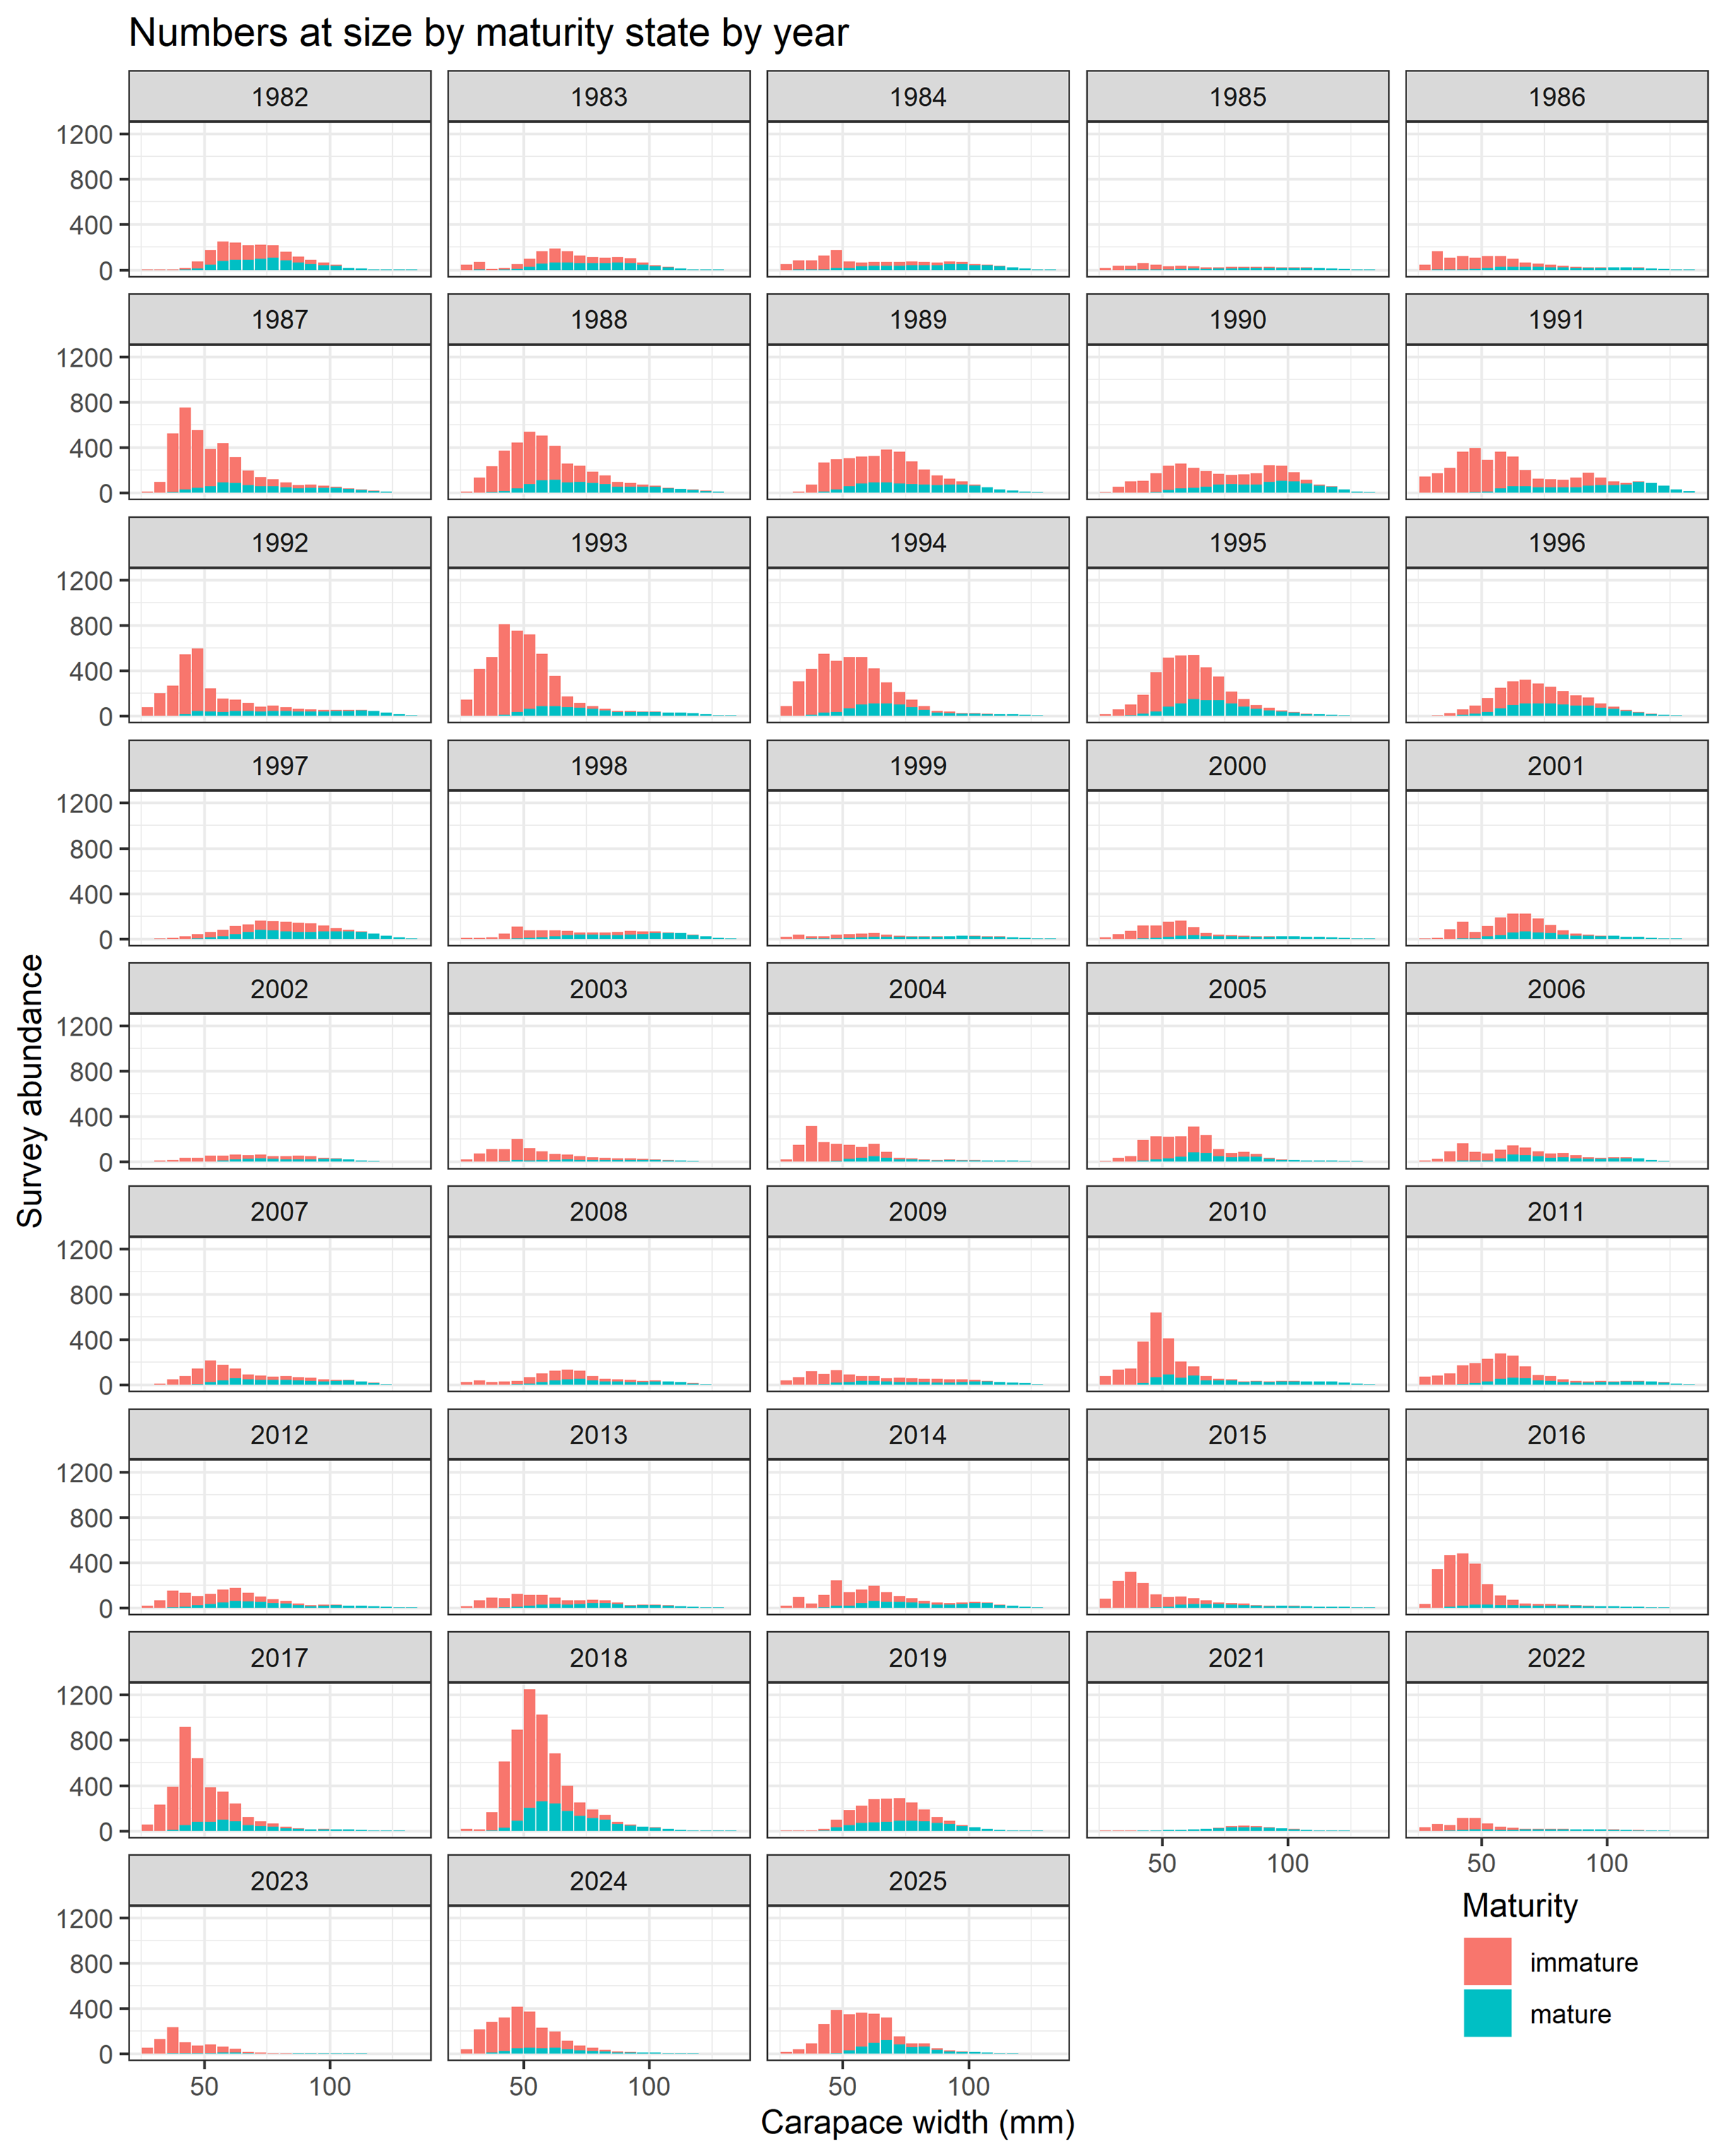
\includegraphics[height=0.65\textheight]{NumbersMaturity.png}
\tiny Numbers of immature/mature crab at size from the survey, by year
(legacy maturity workflow). Updated figure with new survey + new
maturity workflow will be in the September document.
\end{frame}

\begin{frame}{Other SSC items addressed}
\phantomsection\label{other-ssc-items-addressed}
\small

\begin{itemize}
\tightlist
\item
  \textbf{Rebuilding analysis.} Will be added to the September SAFE
  (overfished status was declared in 2021).
\item
  \textbf{Tier 4 fallback} (2024(10) SSC; 2024(6) CPT). Standardized
  Tier 4 fallback (REMA-smoothed total mature male biomass; \(F\) = best
  \(M\) estimate from Tier 3) \textbf{will be presented in September}.
  For reference, 2025 Tier 4 OFLs were 28.41, 8.64, and 6.11 kt for
  morphometric, large (\textgreater=95 mm), and preferred
  (\textgreater101 mm) males.
\item
  \textbf{Maximin / yield-per-recruit} (2024(10), 2025(6) SSC). Maximin
  work was extended in Szuwalski and Punt (2025); steepness values
  0.5/0.67/0.8 do not match available reproductive data. YPR exercise
  was not completed.
\item
  \textbf{Density-dependent maturity / temperature--\(M\) link} (2025(6)
  SSC). Both relationships described in Szuwalski et al.~(2026).
\item
  \textbf{Clutch fullness / reproductive contribution of small males}
  (2025(6) SSC). Preliminary analyses do not show an important link to
  recruitment; CamSled work observed small mature males grasping mature
  females.
\item
  \textbf{VAST / NBS+EBS} (2024(10) SSC). Indices for mature females and
  large males presented to May 2025 CPT; cautious about extrapolating
  into NBS in years without data.
\end{itemize}
\end{frame}

\section{Assessment scenarios}\label{assessment-scenarios}

\begin{frame}[fragile]{Model framework}
\phantomsection\label{model-framework}
Same structural assumptions across all 14 candidates -- differences only
in \textbf{GMACS version, data inputs, maturity ogive, and plus group}.

\smallskip
\small

\begin{itemize}
\tightlist
\item
  Probability of terminal molt at size \textbf{input as data} (varies by
  year and size).
\item
  Survey selectivity estimated by era (1982--88; 1989--present) and sex
  with priors from BSFRF.
\item
  Growth = linear function of pre-molt CW with specified variance.
\item
  Natural mortality estimated by sex/maturity with \textbf{mortality
  events} in 2018 and 2019.
\item
  All immature crab molt; mature crab undergo terminal molt.
\item
  Total and retained fishery selectivity = logistic curves.
\item
  All non-directed bycatch lumped into a single fleet.
\item
  Recruitment estimated separately for males and females; first 3 size
  bins.
\end{itemize}

\smallskip

GMACS \textbf{v2.20.34} (compiled 2026-01-15) for all candidate runs
except \texttt{Model\ 25} (rolled forward).
\end{frame}

\begin{frame}[fragile]{Naming convention -- additive series of changes}
\phantomsection\label{naming-convention-additive-series-of-changes}
\small

\begin{longtable}[]{@{}
  >{\raggedright\arraybackslash}p{(\linewidth - 2\tabcolsep) * \real{0.4706}}
  >{\raggedright\arraybackslash}p{(\linewidth - 2\tabcolsep) * \real{0.5294}}@{}}
\toprule\noalign{}
\begin{minipage}[b]{\linewidth}\raggedright
Suffix
\end{minipage} & \begin{minipage}[b]{\linewidth}\raggedright
Meaning
\end{minipage} \\
\midrule\noalign{}
\endhead
\texttt{update} & Updated GMACS executable (2.20.34) \\
\texttt{compfix} & Total-male comp file corrected to match the script
output \\
\texttt{plus\ group} & Plus group widened to include all crab
\textgreater{} 135 mm CW \\
\texttt{imm\_surv} & Immature survey biomass index added \\
\texttt{new\_mat} & New \texttt{sdmTMB} maturity workflow (Kodiak;
Ryznar in prep) \\
\texttt{hyb\_fishery} & Hybrid catch added to directed-fishery comp /
discards \\
\texttt{hyb\_surv} & Hybrid added to NMFS summer trawl survey biomass /
comp \\
\texttt{hyb\_both} & Hybrids added to both survey and fishery \\
\bottomrule\noalign{}
\end{longtable}

\medskip

\centering Models grouped under \textbf{four axes of uncertainty} in the
next slides.
\end{frame}

\begin{frame}[fragile]{Axis 1 -- Model \& plus-group updates}
\phantomsection\label{axis-1-model-plus-group-updates}
\small

\begin{longtable}[]{@{}
  >{\raggedright\arraybackslash}p{(\linewidth - 2\tabcolsep) * \real{0.3500}}
  >{\raggedright\arraybackslash}p{(\linewidth - 2\tabcolsep) * \real{0.6500}}@{}}
\toprule\noalign{}
\begin{minipage}[b]{\linewidth}\raggedright
Model
\end{minipage} & \begin{minipage}[b]{\linewidth}\raggedright
Description
\end{minipage} \\
\midrule\noalign{}
\endhead
\texttt{Model\ 25} & September 2025 author-recommended; rolled forward
(no updates) \\
\texttt{Model\ 25.1a} & \texttt{Model\ 25} rebuilt with updated GMACS
(2.20.34) \\
\texttt{Model\ 25.1b} & \texttt{25.1a} + correct total-male composition
file (\texttt{compfix}) \\
\texttt{Model\ 25.1c} & \texttt{25.1b} + plus group at \textgreater135
mm CW (retained: 278/2,239; total: 422/3,151; female discard:
1/1,175) \\
\bottomrule\noalign{}
\end{longtable}

\medskip

\begin{itemize}
\tightlist
\item
  The \textbf{plus-group change makes the model run substantially
  faster} (23 min vs.~29 min) and is the \textbf{structural baseline}
  for most sensitivities.
\item
  Compfix reconciles a small file discrepancy from September 2025.
\end{itemize}
\end{frame}

\begin{frame}[fragile]{Axis 2 -- Immature survey index}
\phantomsection\label{axis-2-immature-survey-index}
\small

\begin{longtable}[]{@{}ll@{}}
\toprule\noalign{}
Model & Description \\
\midrule\noalign{}
\endhead
\texttt{Model\ 25.1d} & \texttt{25.1b} + immature survey biomass
index \\
\texttt{Model\ 25.1e} & \texttt{25.1c} + immature survey biomass
index \\
\bottomrule\noalign{}
\end{longtable}

\medskip

\begin{itemize}
\tightlist
\item
  Immature index provides \textbf{direct information on immature
  abundance}.
\item
  \textbf{Removes the bimodality} observed in jitter analyses (see
  Results).
\item
  Comes with a \textbf{substantially higher estimate of mature male
  \(M\)} that propagates into reference points and reduces \(B_{MSY}\).
\item
  Combination of immature index + hybrids was \textbf{not explored}.
\end{itemize}
\end{frame}

\begin{frame}[fragile]{Axis 3 -- New maturity workflow (Kodiak /
Ryznar)}
\phantomsection\label{axis-3-new-maturity-workflow-kodiak-ryznar}
\small

\begin{longtable}[]{@{}ll@{}}
\toprule\noalign{}
Model & Description \\
\midrule\noalign{}
\endhead
\texttt{Model\ 25.2a} & \texttt{25.1a} + new maturity ogive \\
\texttt{Model\ 25.2b} & \texttt{25.1b} + new maturity ogive \\
\texttt{Model\ 25.2c} & \texttt{25.1c} + new maturity ogive \\
\texttt{Model\ 25.2d} & \texttt{25.1c} + new maturity + immature
survey \\
\bottomrule\noalign{}
\end{longtable}

\medskip

\begin{itemize}
\tightlist
\item
  New workflow: \textbf{\texttt{sdmTMB} spatiotemporal model} fit to
  chela-based maturity classifications.
\item
  Borrows information across years and locations; does \textbf{not
  extrapolate} beyond stations with measured crab.
\item
  New workflow has a \textbf{much weaker temporal trend} in
  \(\Pr\)(terminal molt) at intermediate sizes (e.g., at 77 mm) than the
  legacy workflow.
\item
  Updates affect mature male survey abundance and male composition data;
  female time series unchanged.
\end{itemize}
\end{frame}

\begin{frame}[fragile]{Axis 4 -- Hybrid treatment}
\phantomsection\label{axis-4-hybrid-treatment}
\small

\begin{longtable}[]{@{}
  >{\raggedright\arraybackslash}p{(\linewidth - 2\tabcolsep) * \real{0.3500}}
  >{\raggedright\arraybackslash}p{(\linewidth - 2\tabcolsep) * \real{0.6500}}@{}}
\toprule\noalign{}
\begin{minipage}[b]{\linewidth}\raggedright
Model
\end{minipage} & \begin{minipage}[b]{\linewidth}\raggedright
Description
\end{minipage} \\
\midrule\noalign{}
\endhead
\texttt{Model\ 25.3a} & \texttt{25.1c} + hybrids in directed-fishery
comp + discards \\
\texttt{Model\ 25.3b} & \texttt{25.1c} + hybrids in NMFS summer survey
biomass + comp \\
\texttt{Model\ 25.3c} & \texttt{25.1c} + hybrids in both survey and
fishery \\
\texttt{Model\ 25.3d} & \texttt{25.3c} + new maturity workflow \\
\bottomrule\noalign{}
\end{longtable}

\medskip

\begin{itemize}
\tightlist
\item
  ADF\&G provided hybrid data as a \textbf{separate species code}
  (lumped opilio-, bairdi-, and unspecified-type).
\item
  Hybrid weights computed using \textbf{snow crab L--W parameters} (most
  hybrids are opilio-type).
\item
  Hybrid data are \textbf{additive} to existing snow-crab time series,
  \textbf{except retained catch} (hybrids already retained under snow
  IFQ; cannot be separated).
\item
  CV on directed discards held at 0.7. Observer non-directed bycatch
  unchanged.
\end{itemize}
\end{frame}

\section{Data comparisons across
scenarios}\label{data-comparisons-across-scenarios}

\begin{frame}{NMFS survey biomass index -- mature crab}
\phantomsection\label{nmfs-survey-biomass-index-mature-crab}
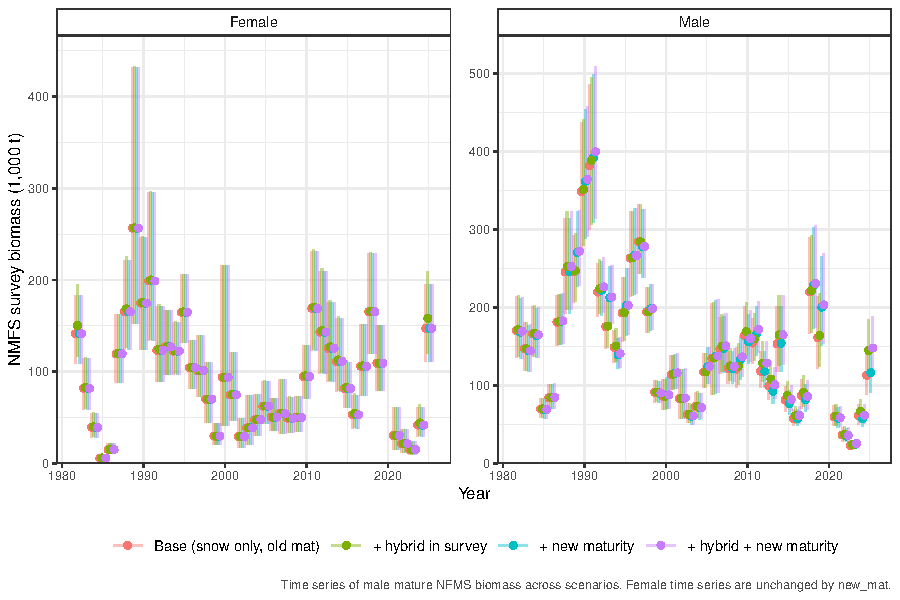
\includegraphics[width=1\linewidth,height=\textheight,keepaspectratio]{Snow2026_may_CPT_files/figure-beamer/idx-mature-1.pdf}
\end{frame}

\begin{frame}{NMFS survey biomass index -- immature crab}
\phantomsection\label{nmfs-survey-biomass-index-immature-crab}
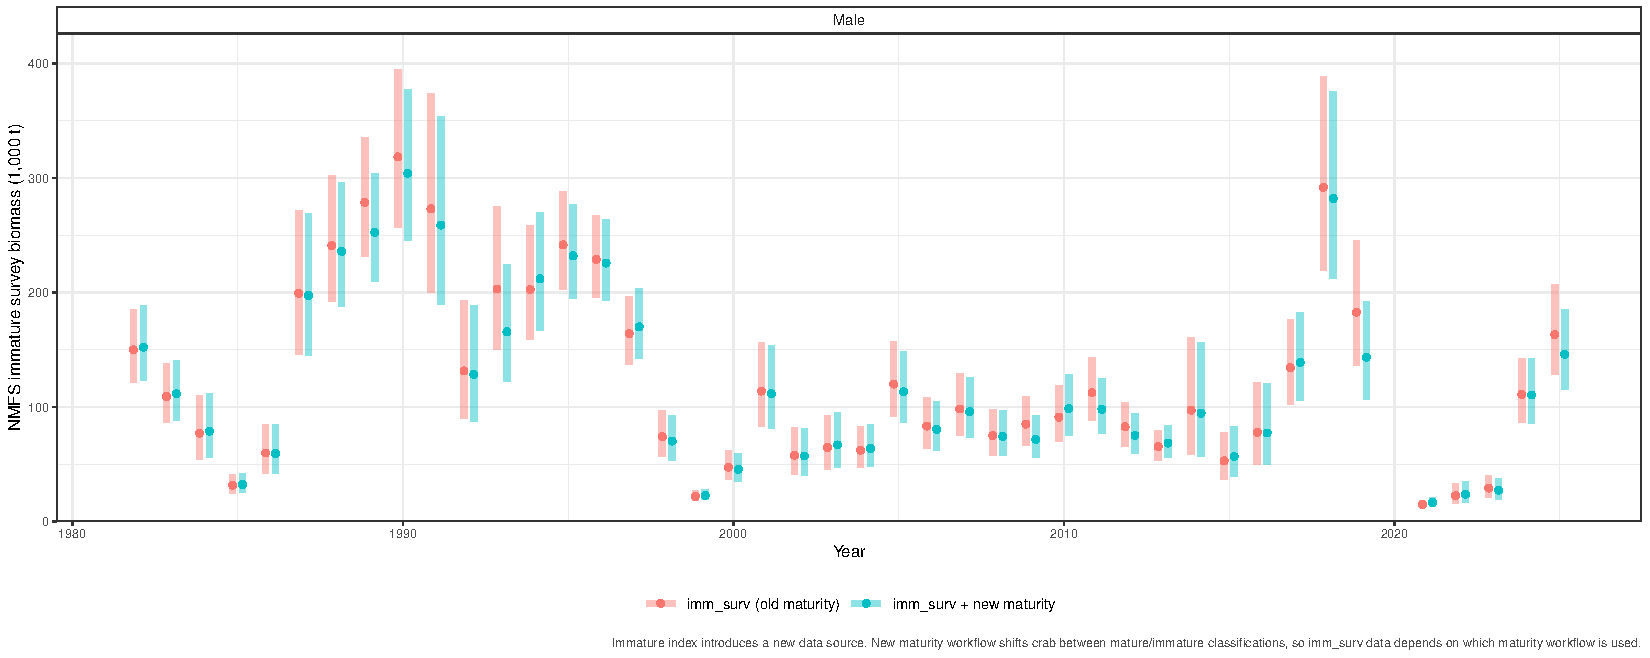
\includegraphics[width=1\linewidth,height=\textheight,keepaspectratio]{Snow2026_may_CPT_files/figure-beamer/idx-imm-1.pdf}
\end{frame}

\begin{frame}{Catch data -- retained, discards, bycatch}
\phantomsection\label{catch-data-retained-discards-bycatch}
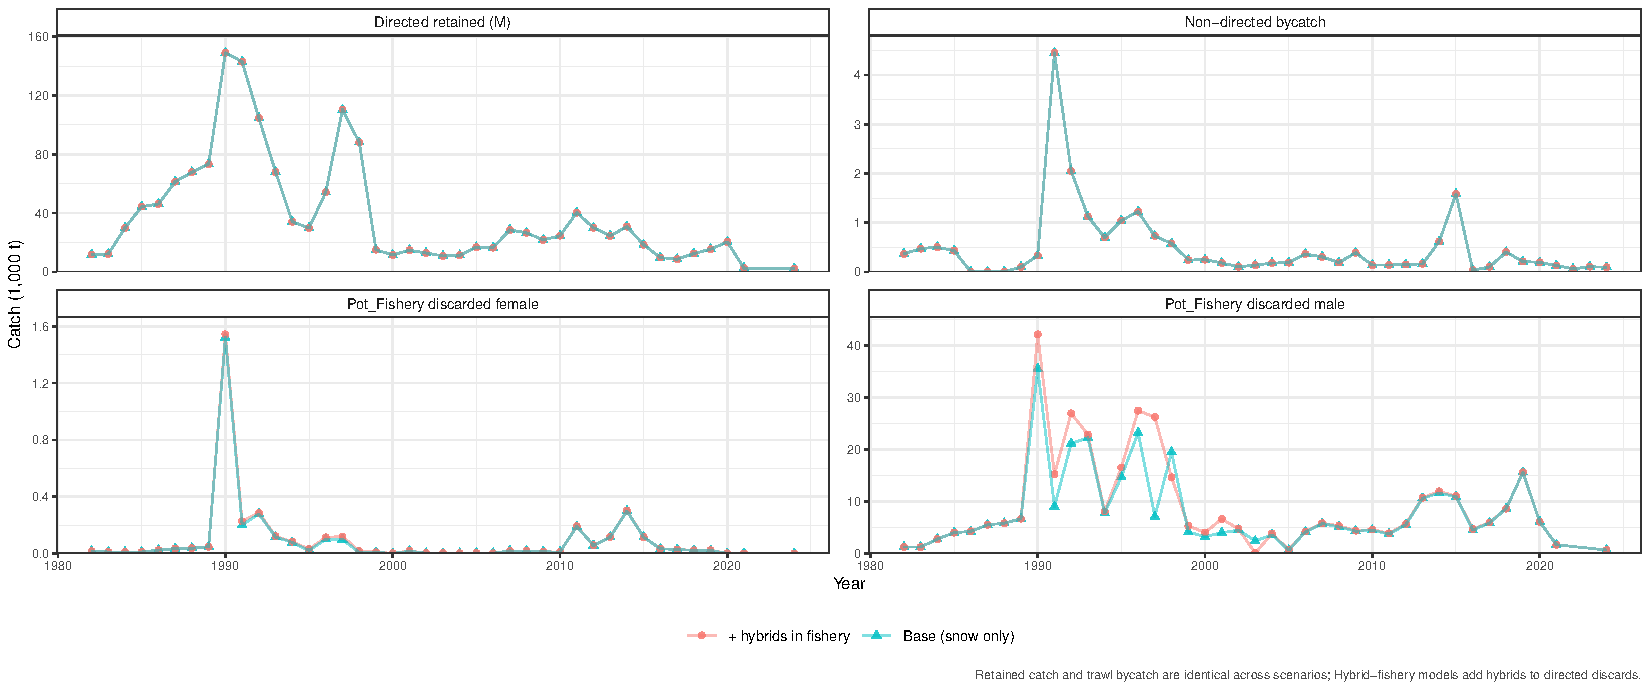
\includegraphics[width=1\linewidth,height=\textheight,keepaspectratio]{Snow2026_may_CPT_files/figure-beamer/catch-compare-1.pdf}
\end{frame}

\begin{frame}{Pot fishery composition -- compfix vs.~plus group
vs.~hybrid}
\phantomsection\label{pot-fishery-composition-compfix-vs.-plus-group-vs.-hybrid}
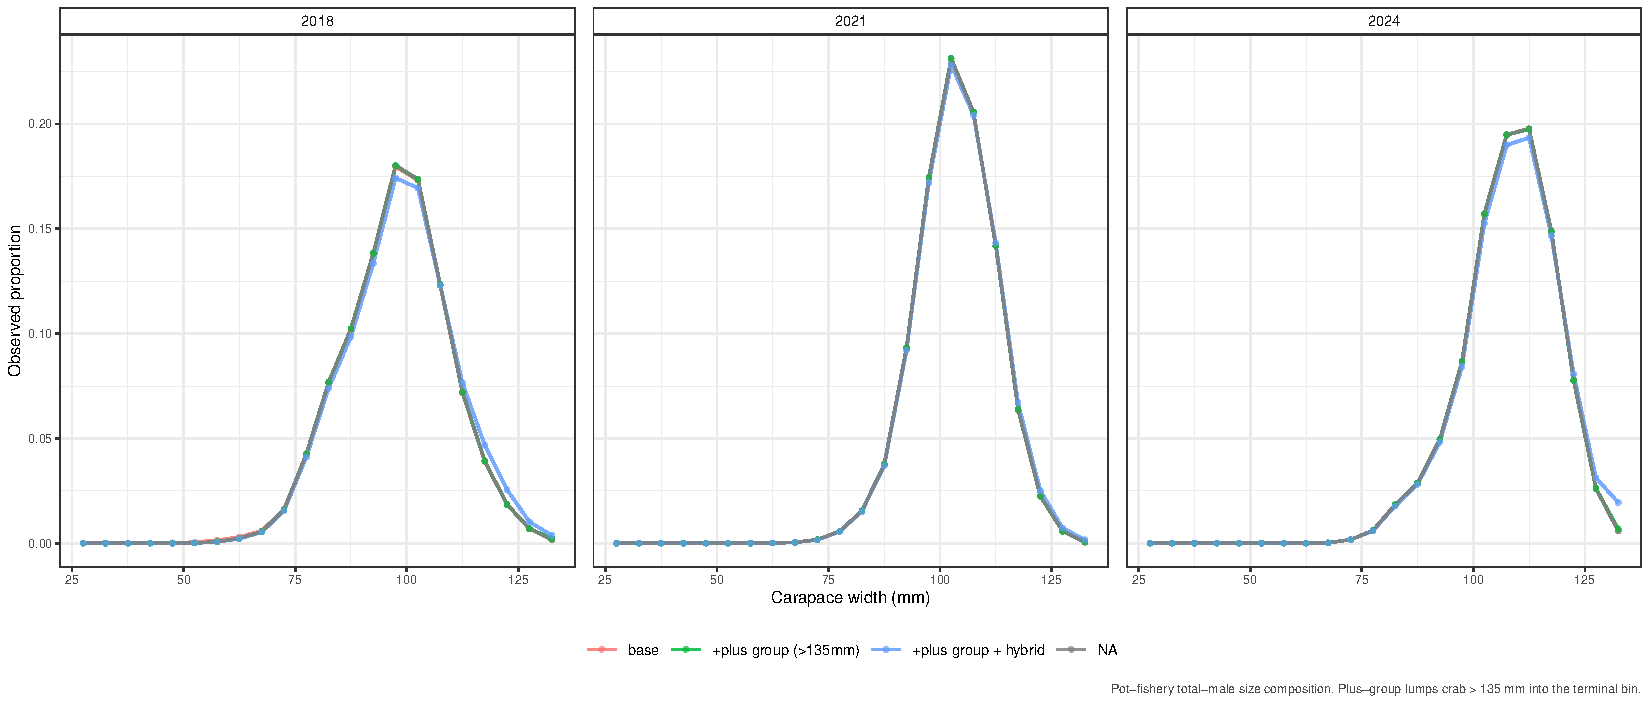
\includegraphics[width=1\linewidth,height=\textheight,keepaspectratio]{Snow2026_may_CPT_files/figure-beamer/comp-pot-1.pdf}
\end{frame}

\begin{frame}{NMFS survey composition -- hybrid vs.~new maturity}
\phantomsection\label{nmfs-survey-composition-hybrid-vs.-new-maturity}
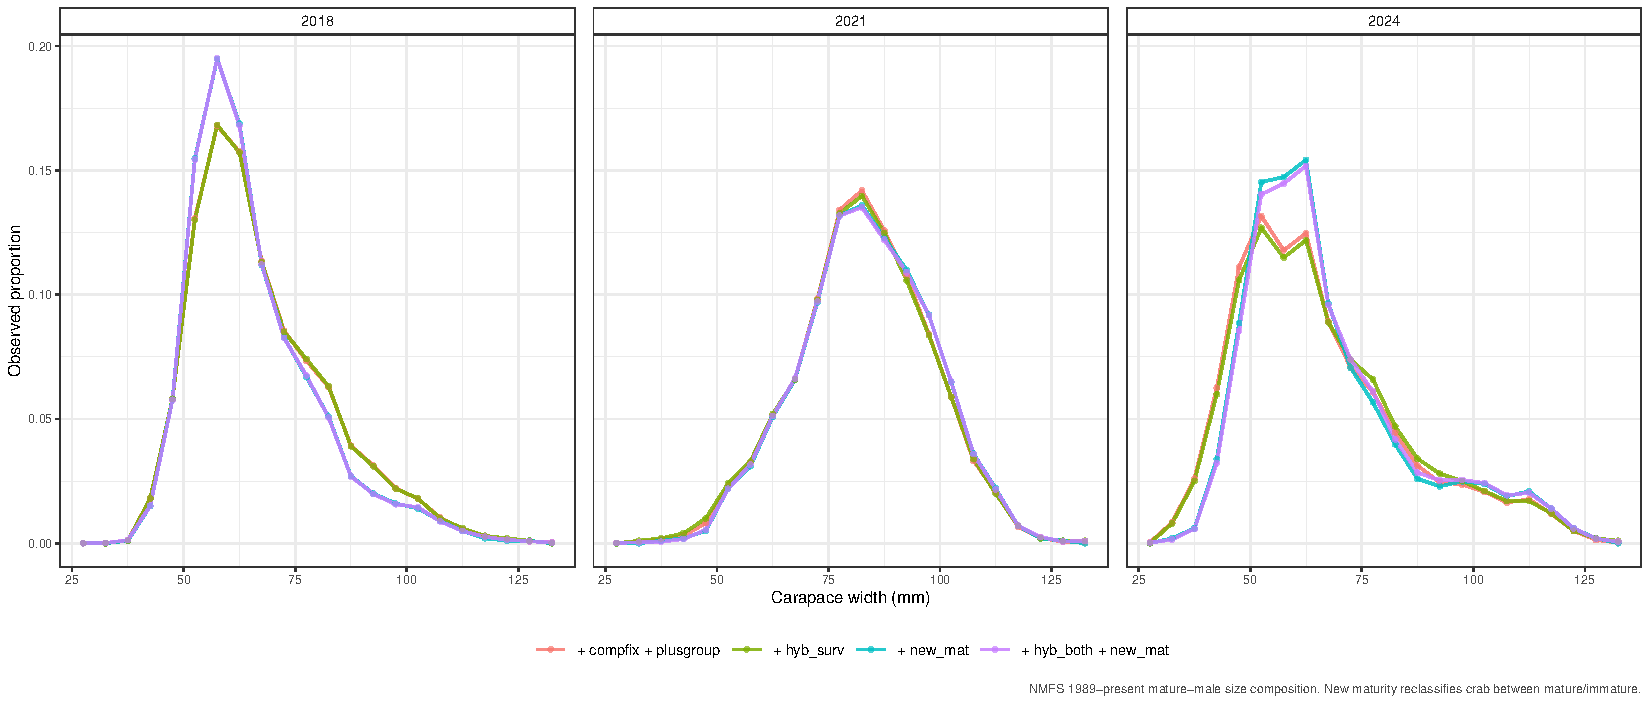
\includegraphics[width=1\linewidth,height=\textheight,keepaspectratio]{Snow2026_may_CPT_files/figure-beamer/comp-survey-1.pdf}
\end{frame}

\begin{frame}{Pot fishery female discard composition}
\phantomsection\label{pot-fishery-female-discard-composition}
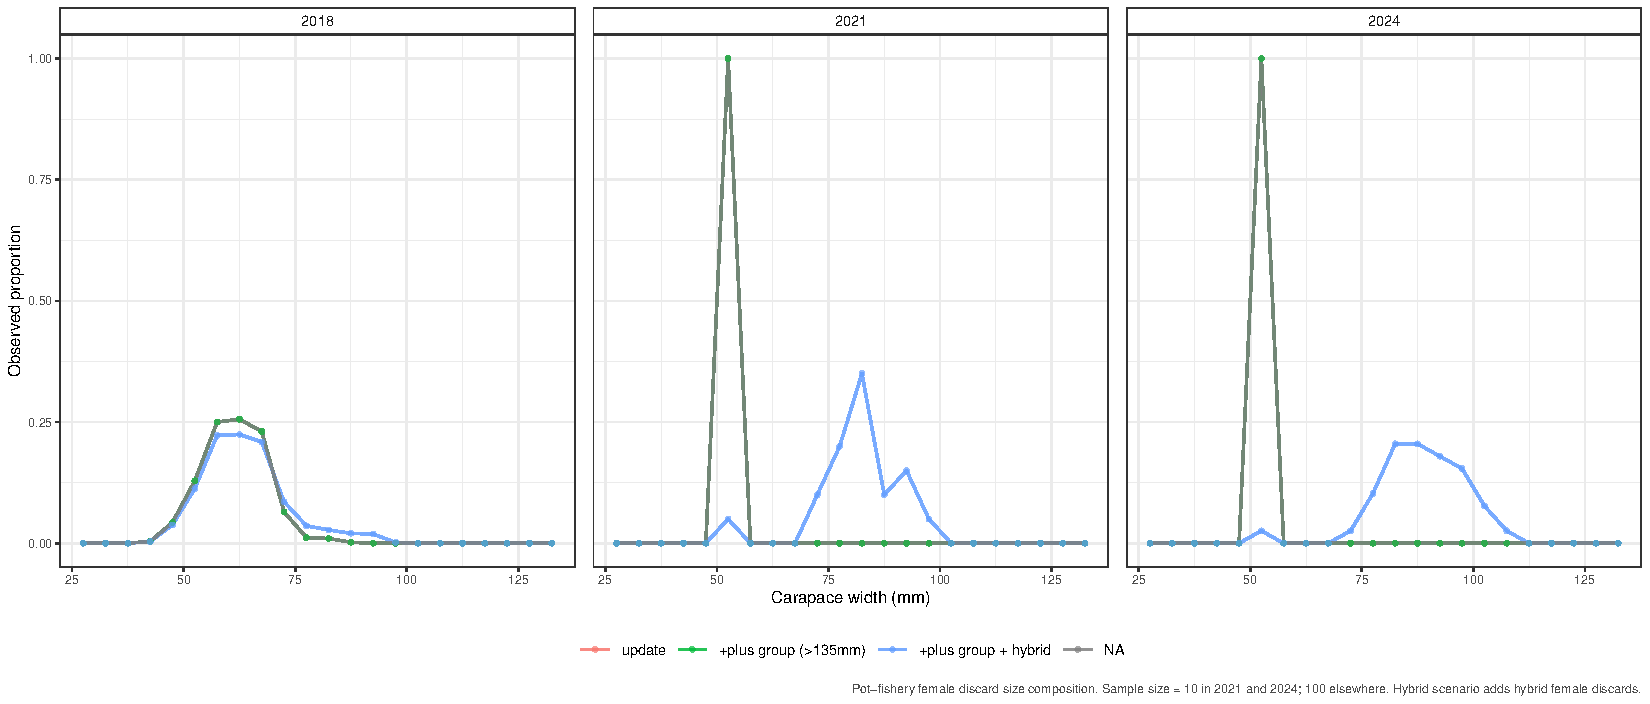
\includegraphics[width=1\linewidth,height=\textheight,keepaspectratio]{Snow2026_may_CPT_files/figure-beamer/comp-pot-fem-1.pdf}
\end{frame}

\begin{frame}{Maturity ogive -- legacy vs.~new workflow}
\phantomsection\label{maturity-ogive-legacy-vs.-new-workflow}
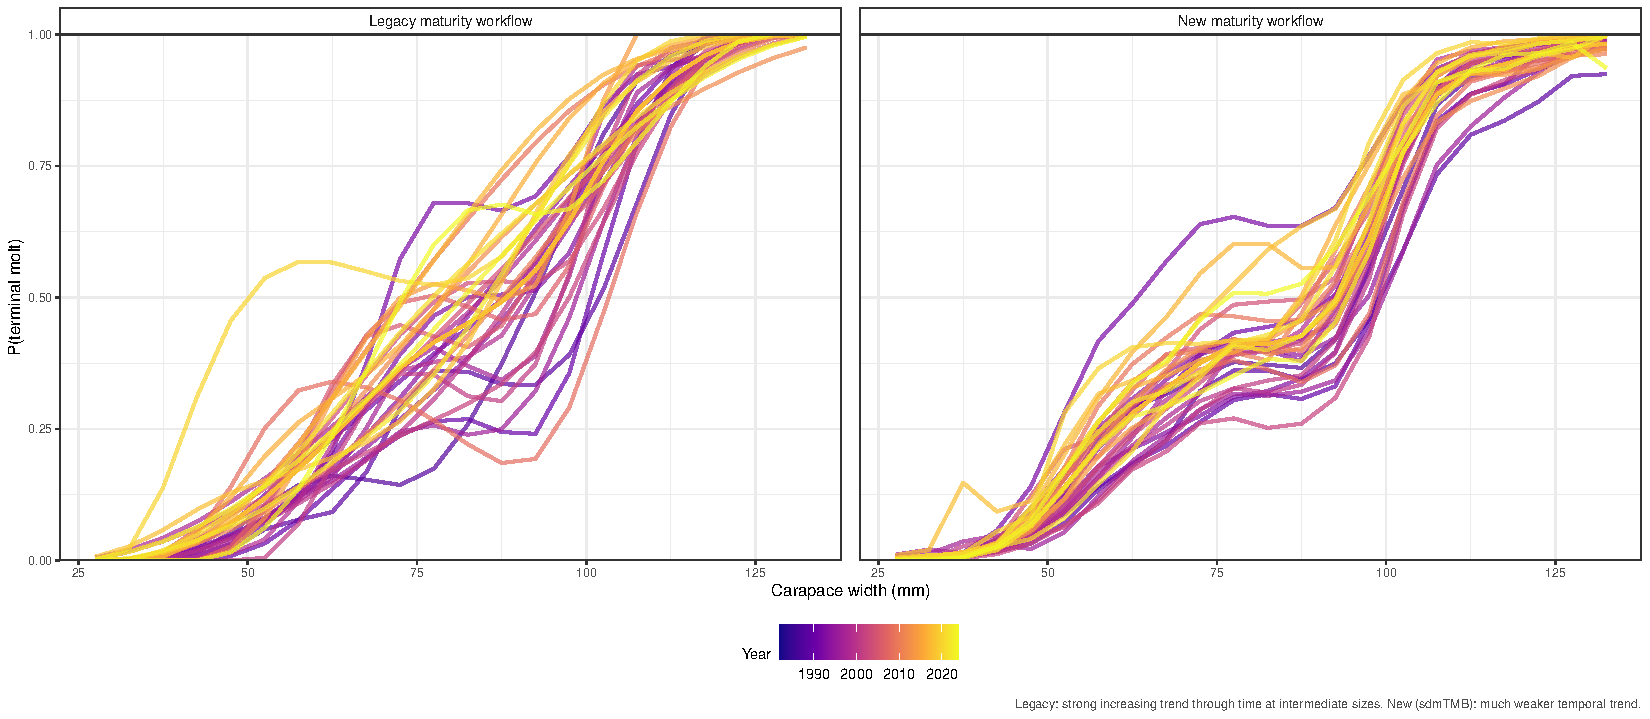
\includegraphics[width=1\linewidth,height=\textheight,keepaspectratio]{Snow2026_may_CPT_files/figure-beamer/predmat-ogive-1.pdf}
\end{frame}

\begin{frame}{P(mature) over time at fixed sizes -- 50, 80, 101 mm}
\phantomsection\label{pmature-over-time-at-fixed-sizes-50-80-101-mm}
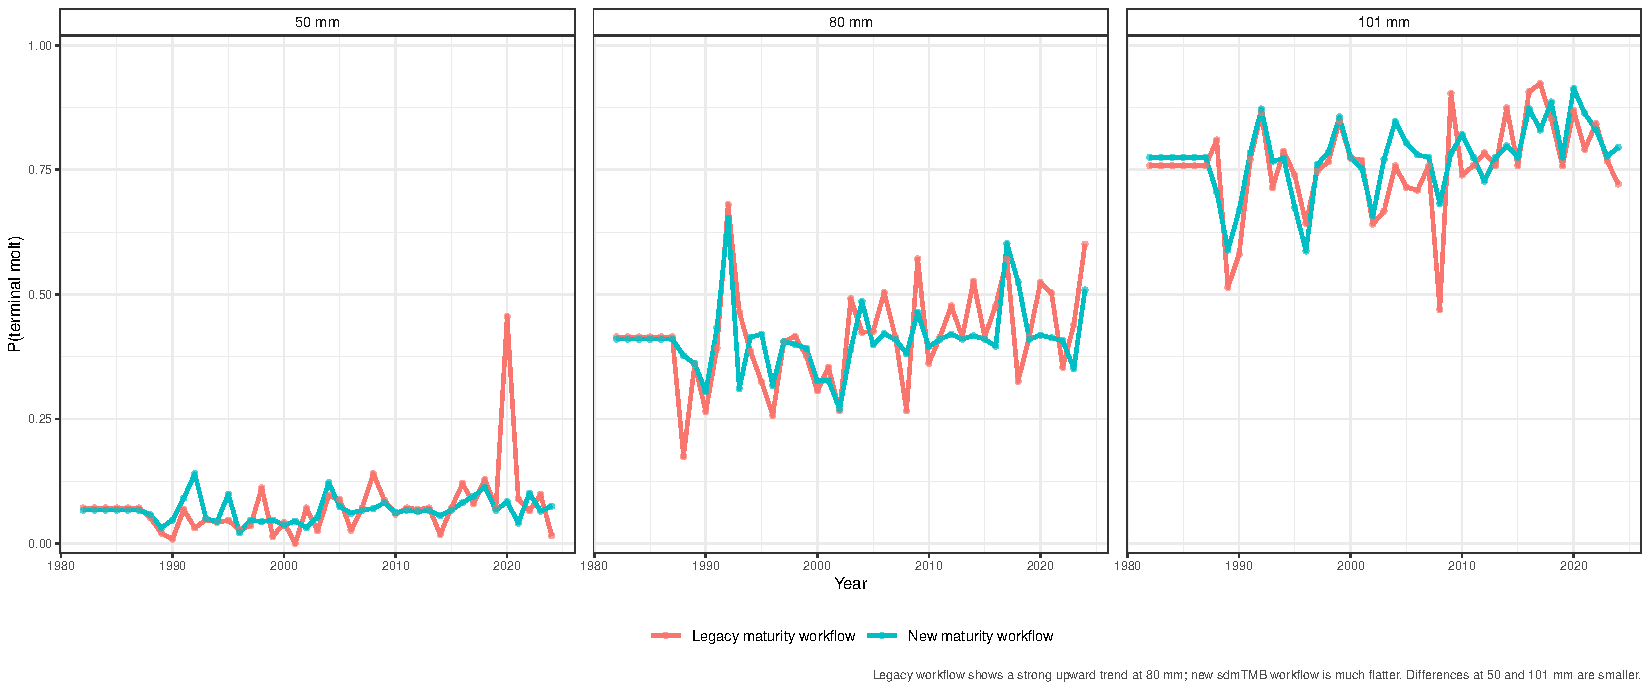
\includegraphics[width=1\linewidth,height=\textheight,keepaspectratio]{Snow2026_may_CPT_files/figure-beamer/predmat-timeseries-1.pdf}
\end{frame}

\section{Data updates}\label{data-updates}

\begin{frame}[fragile]{Total male composition fix (compfix)}
\phantomsection\label{total-male-composition-fix-compfix}
\begin{itemize}
\tightlist
\item
  Small discrepancy between the file used in the September 2025
  assessment and the version produced by the script that translates the
  ADF\&G files.
\item
  Reconciled by re-running the translation script
  (\texttt{tot\_sc\_m.csv}) and replacing the affected total-male
  composition entries.
\item
  Effect on management quantities is small but \textbf{internally
  consistent files are required}.
\end{itemize}

\centering

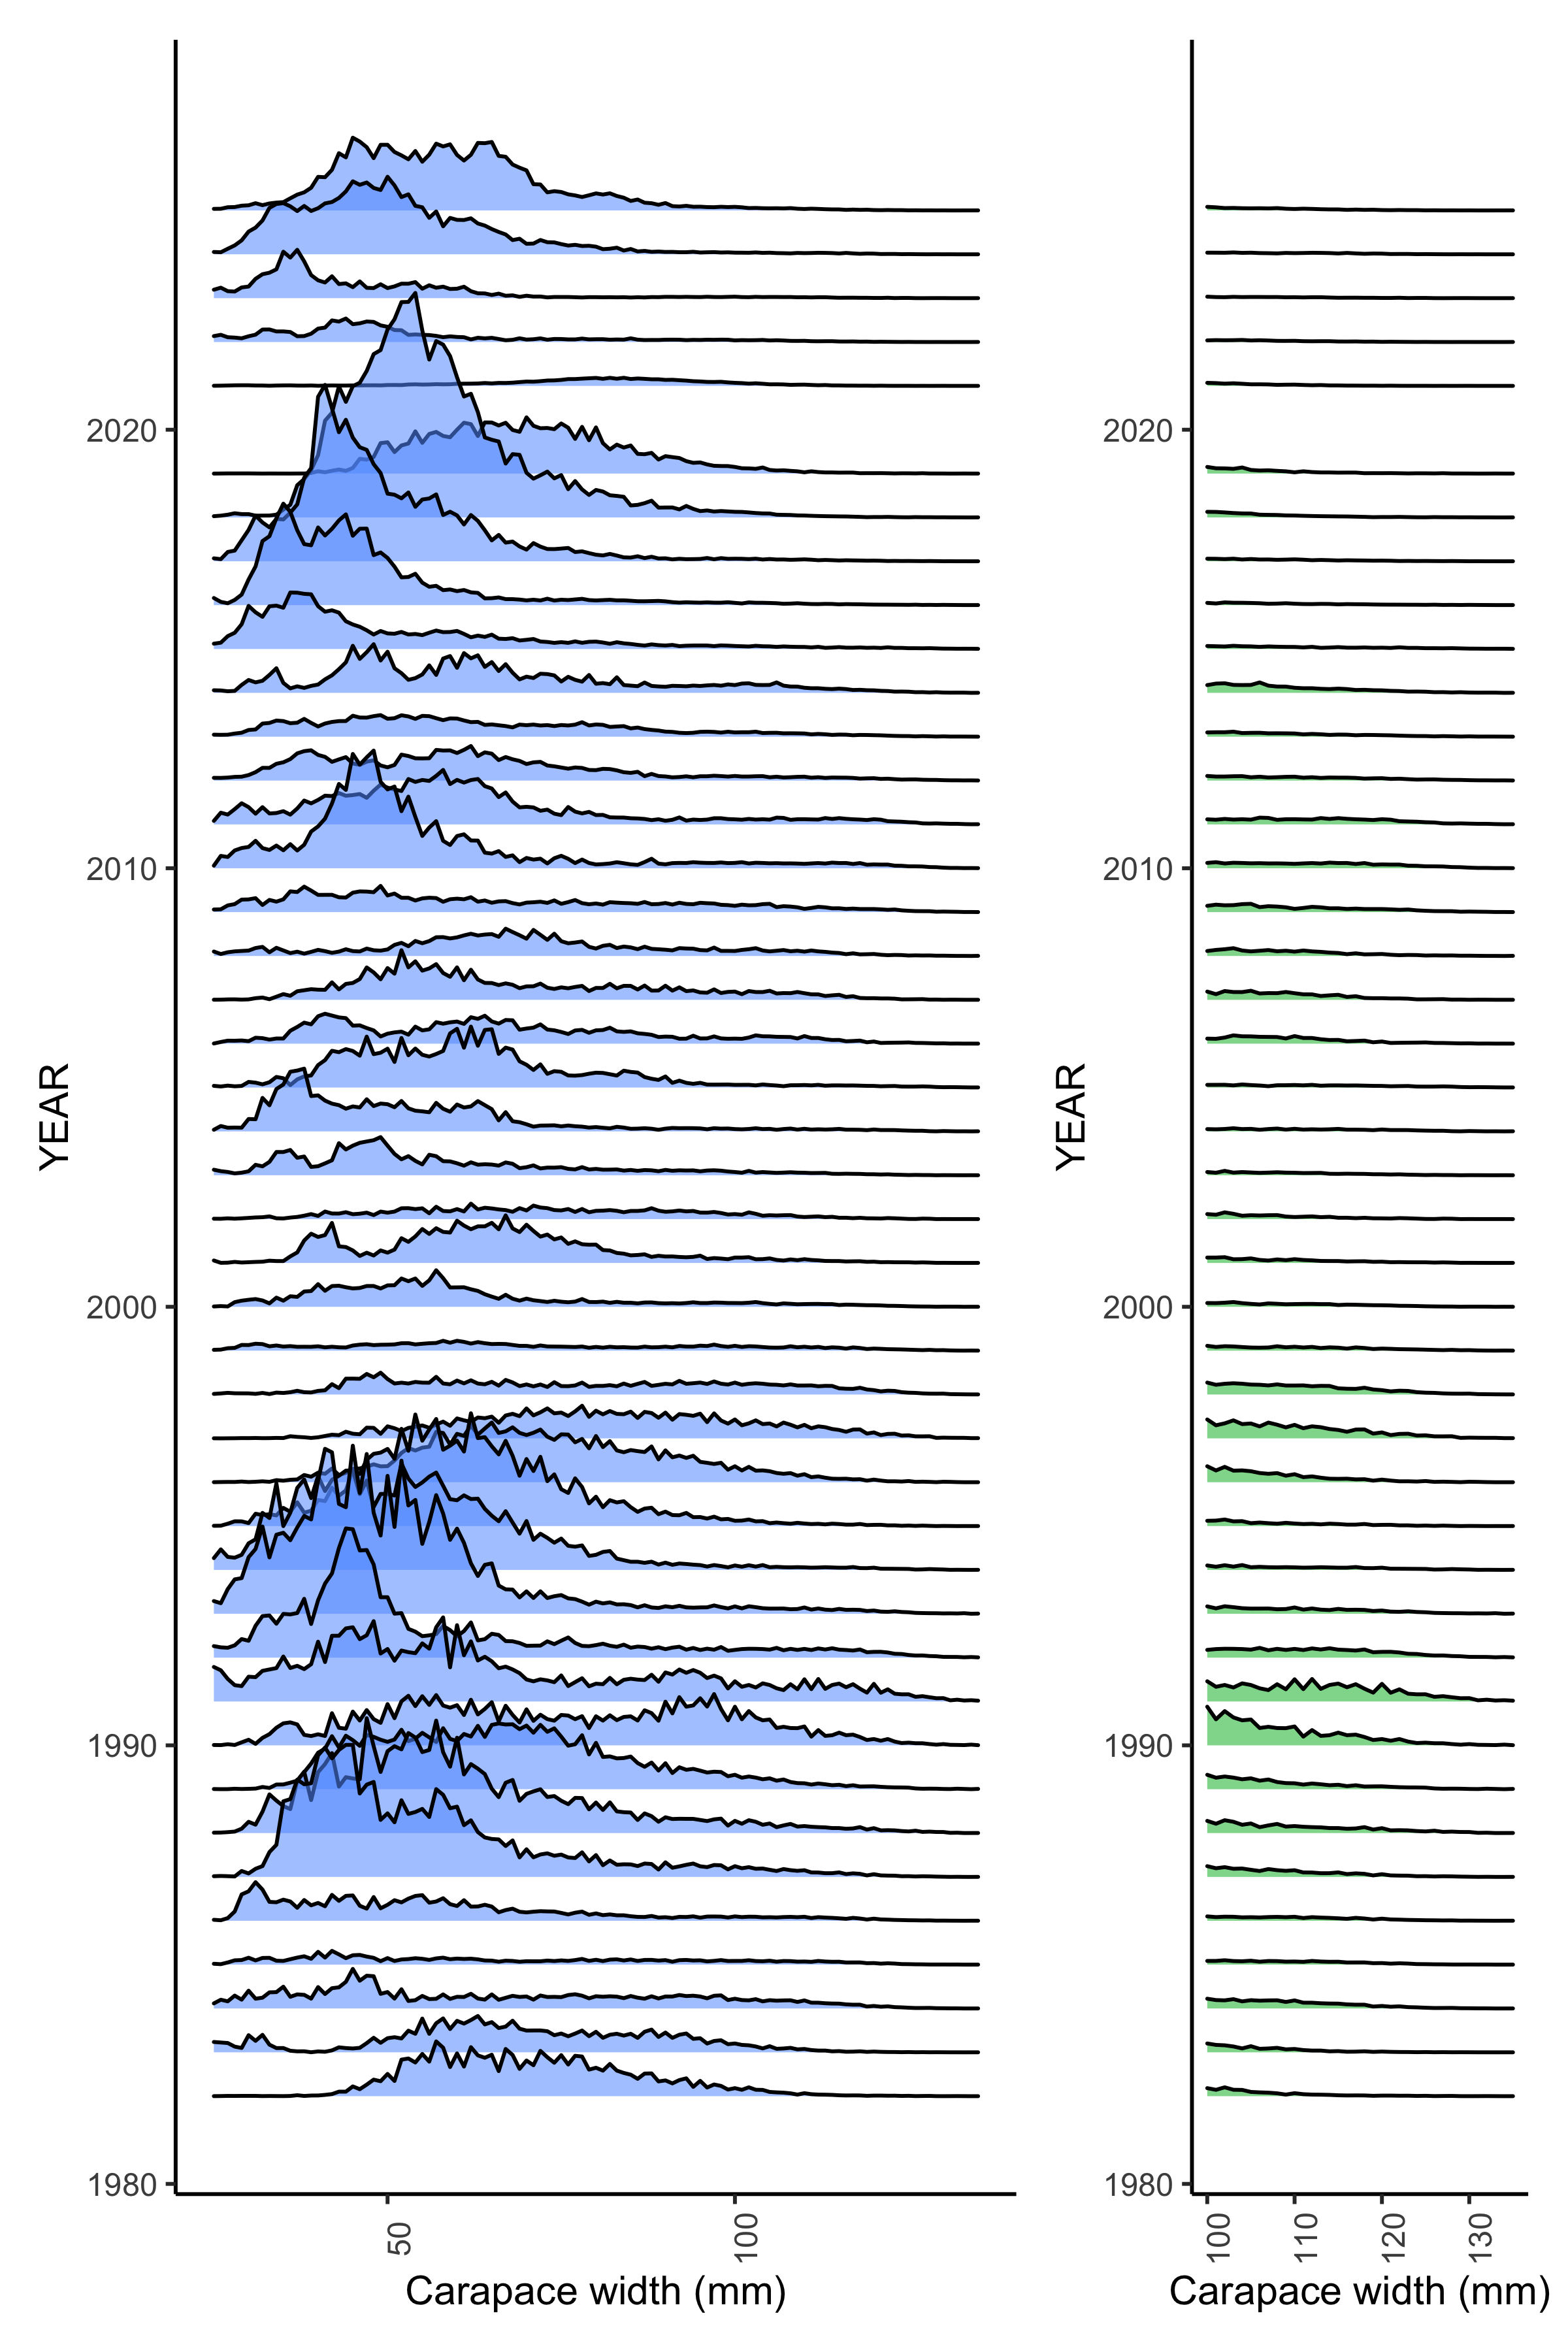
\includegraphics[height=0.5\textheight]{plots/size_bins_comp_Kodiak_m.png}
\tiny Total-male size composition data (compfix) by size bin.
\end{frame}

\begin{frame}{Plus group at \textgreater135 mm CW}
\phantomsection\label{plus-group-at-135-mm-cw}
\begin{columns}[T]
\begin{column}{0.6\linewidth}
\small

\begin{itemize}
\tightlist
\item
  Previous model \textbf{ignored crab \textgreater{} 135 mm}.
\item
  Updated plus group lumps all crab \textgreater{} 135 mm into a single
  bin for:

  \begin{itemize}
  \tightlist
  \item
    Retained males (n = 278 of 2,239 samples)
  \item
    Total males (n = 422 of 3,151 samples)
  \item
    Discard females (n = 1 of 1,175 samples)
  \end{itemize}
\item
  \textbf{Improves runtime substantially} (23 min vs.~29 min for the
  comparable model).
\item
  Visual fits at the largest sizes are more interpretable.
\item
  Management quantities change very little.
\end{itemize}
\end{column}

\begin{column}{0.4\linewidth}
\centering

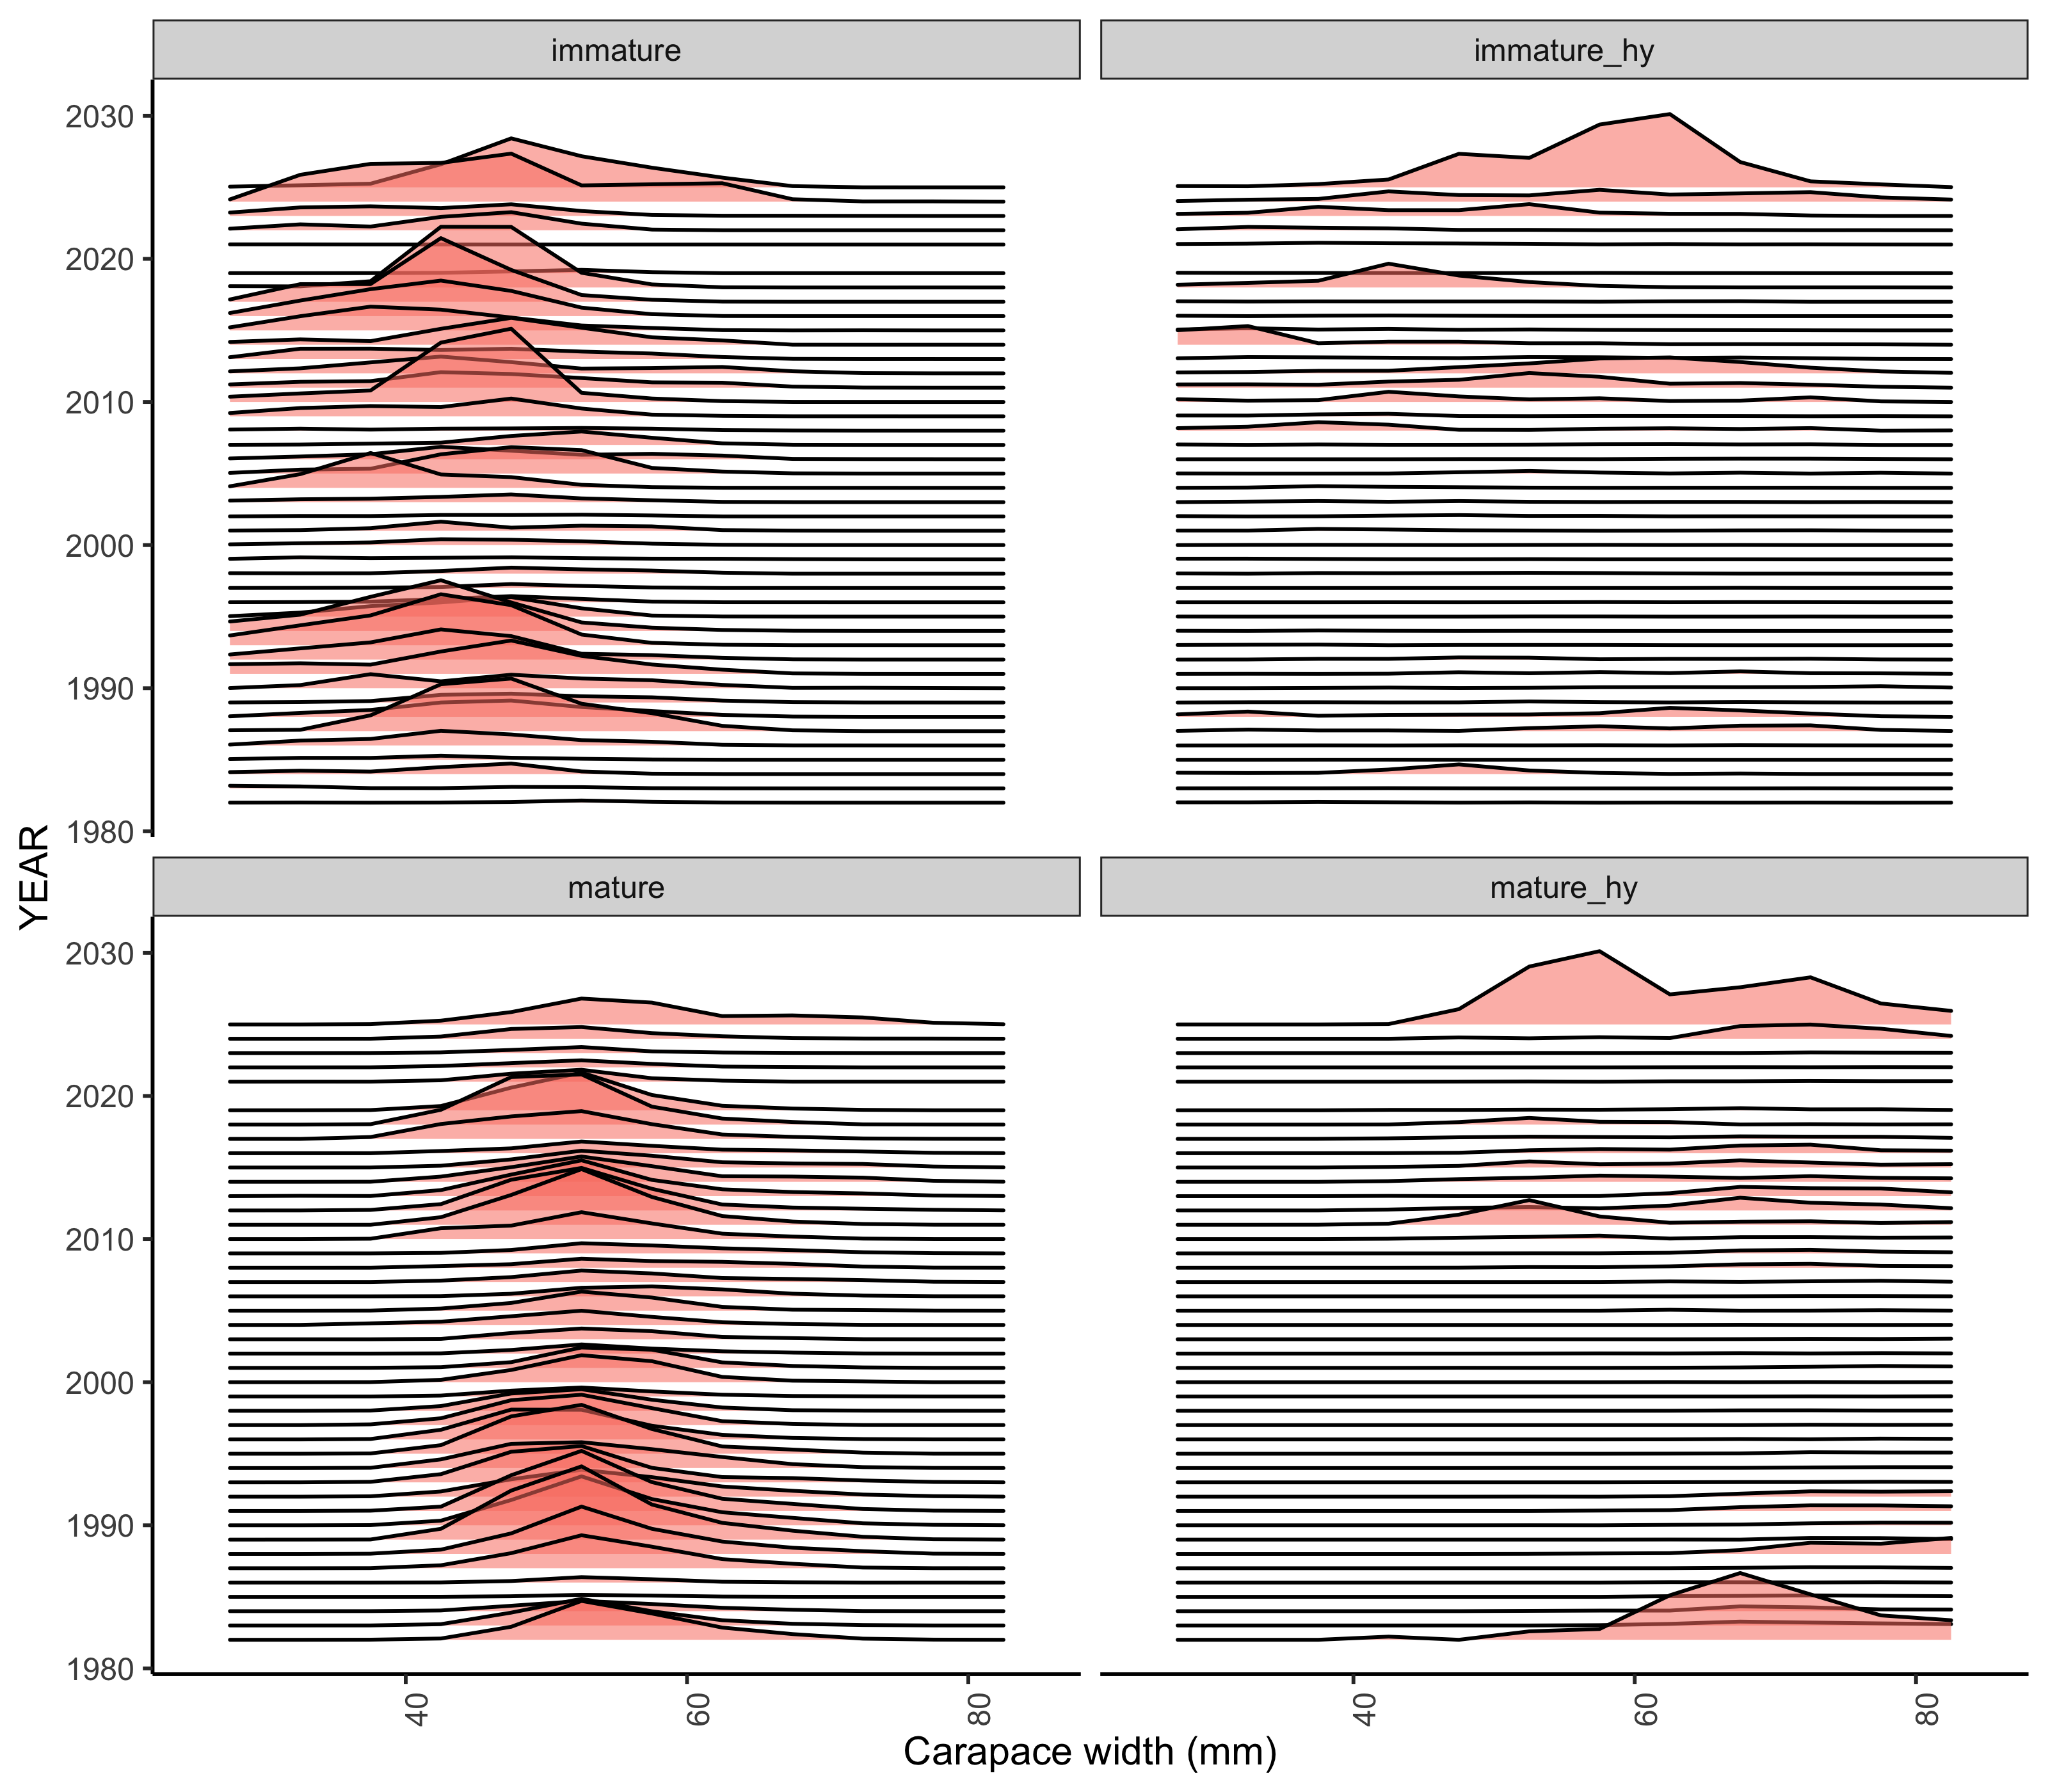
\includegraphics[width=\linewidth]{plots/n_at_l_f.png} \tiny Numbers at
length, females -- illustrates the tail of crab \textgreater{} 135 mm
now retained in the model.
\end{column}
\end{columns}
\end{frame}

\begin{frame}{Hybrid data: directed-fishery discards}
\phantomsection\label{hybrid-data-directed-fishery-discards}
\begin{columns}[T]
\begin{column}{0.55\linewidth}
\small

\begin{itemize}
\tightlist
\item
  ADF\&G provided directed-fishery discards lumped across all hybrid
  types.
\item
  Adding hybrids to the directed pot fishery \textbf{increases discards}
  in some years -- e.g.~legal-male hybrid catch \textasciitilde18 kt in
  1997 and \textasciitilde15 kt in 1998 (flagged by ADF\&G as needing
  QC).
\item
  Models accommodate the added discards primarily through changes in
  \textbf{estimated discard fishing mortality}, not selectivity.
\item
  Retained hybrids cannot be separated from retained snow crab.
\end{itemize}
\end{column}

\begin{column}{0.45\linewidth}
\centering

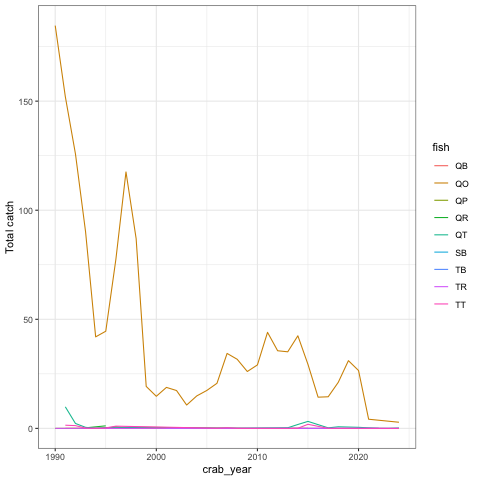
\includegraphics[width=\linewidth]{plots/male_discards.png}
\tiny Observed male discards in the directed pot fishery: snow only
vs.~snow + hybrids.
\end{column}
\end{columns}
\end{frame}

\begin{frame}[fragile]{Hybrid data: NMFS summer trawl survey}
\phantomsection\label{hybrid-data-nmfs-summer-trawl-survey}
\small

\begin{itemize}
\tightlist
\item
  Hybrid catch and composition data added to the NMFS summer trawl
  time-series for \texttt{Models\ 25.3b}, \texttt{25.3c},
  \texttt{25.3d}.
\item
  Visibly \textbf{higher predicted survey biomass} in some years
  (additional hybrid biomass added on top of snow crab); trend through
  time is unchanged.
\item
  Hybrid identification quality \textbf{decreases further back} in the
  time series (consistency between ADF\&G and NMFS criteria is currently
  a research priority).
\end{itemize}

\medskip

\centering

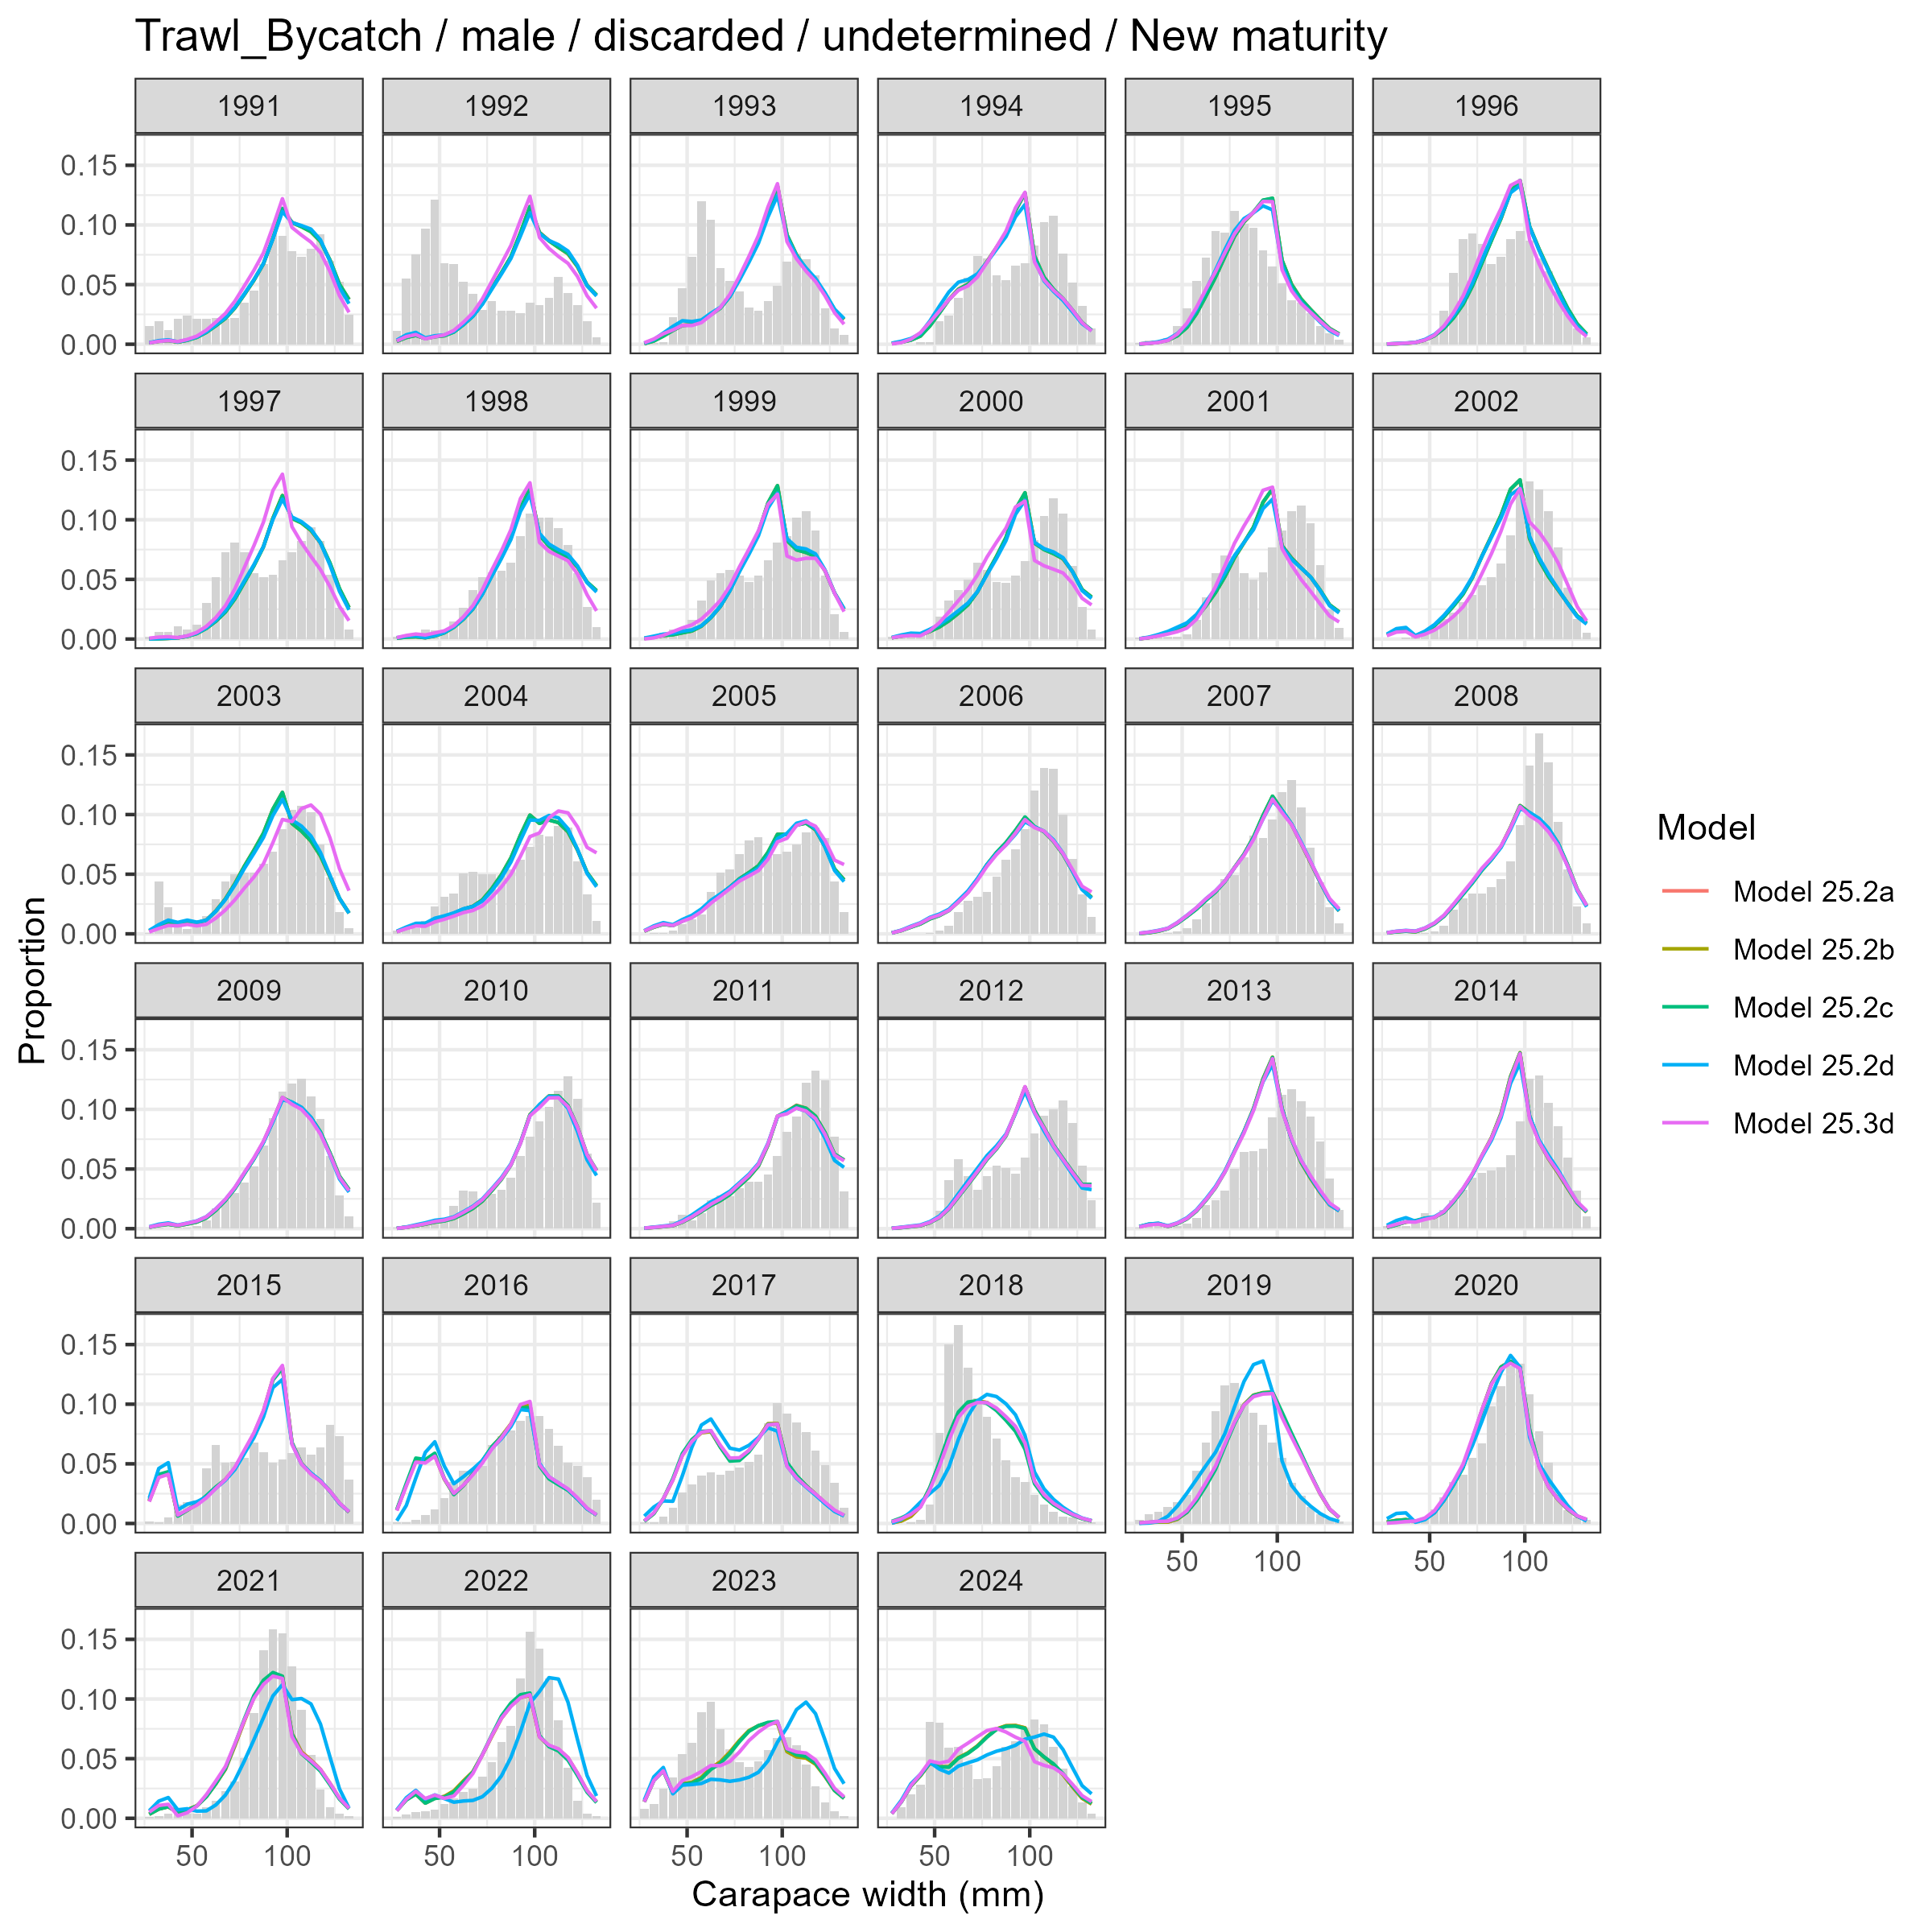
\includegraphics[height=0.45\textheight]{plots/size_comp_plot_46_Trawl_Bycatch_male_discarded_undetermined_New_maturity.png}
\tiny Example survey total-male composition fits for hybrid
vs.~non-hybrid models.
\end{frame}

\begin{frame}[fragile]{New maturity workflow (Kodiak / Ryznar, in prep)}
\phantomsection\label{new-maturity-workflow-kodiak-ryznar-in-prep}
\small

\begin{itemize}
\tightlist
\item
  Replaces the legacy ``fit a curve to chela ratios per year/size''
  approach with a single \textbf{\texttt{sdmTMB} spatiotemporal model}
  fit to chela maturity classifications across all years and stations.
\item
  Borrows information across years and locations for size bins with
  sparse chela data.
\item
  Does not extrapolate the predicted spatial probability surface beyond
  stations with measured crab.
\item
  Population-level annual ogive obtained by integrating the predicted
  surface across stations.
\item
  \textbf{Result:} much weaker temporal trend in \(\Pr\)(terminal molt)
  at intermediate sizes.

  \begin{itemize}
  \tightlist
  \item
    Legacy: at 77 mm, \textasciitilde0.2 (early 1990s) \(\rightarrow\)
    \textasciitilde0.5 (post-2010).
  \item
    New: \textasciitilde0.35--0.45 throughout the time series.
  \end{itemize}
\item
  Updated time series of mature male survey abundance and
  immature/mature comp data; female time series unchanged.
\item
  Sample sizes and CVs of the dependent data \textbf{were not adjusted}
  -- a known limitation.
\end{itemize}
\end{frame}

\section{Convergence and jitter
analysis}\label{convergence-and-jitter-analysis}

\begin{frame}[fragile]{Convergence summary}
\phantomsection\label{convergence-summary}
\small

\begin{itemize}
\tightlist
\item
  All 14 models \textbf{inverted their Hessians}.
\item
  \textbf{Only \texttt{Model\ 25.1d}} met the conventional threshold of
  max \textbar gradient\textbar{} \textless{} 0.001.
\item
  Remaining 13 models had max \textbar gradient\textbar{} \textgreater{}
  0.001; \texttt{Model\ 25.3c} largest at \textasciitilde0.10.
\item
  \textbf{No consistent parameter} had the highest gradient across
  models.
\item
  Likelihood components by category summarized in Tables 2--4 of the
  document.
\end{itemize}

\medskip

\centering

\textbf{Recommendation:} simplify the model where possible (male-only,
fix \(M\) at the prior mean, simpler survey selectivity) and seek
CPT/SSC guidance on what to drop.
\end{frame}

\begin{frame}[fragile]{Jitter analysis -- 100 starts on six models}
\phantomsection\label{jitter-analysis-100-starts-on-six-models}
\small

\begin{itemize}
\tightlist
\item
  Models jittered: \texttt{25.1c}, \texttt{25.1e}, \texttt{25.2c},
  \texttt{25.2d}, \texttt{25.3c}, \texttt{25.3d} (covering all four
  axes).
\item
  Parameter values jittered as \(N(1, 0.1)\) scaled to parameter bounds.
\item
  \textbf{Bimodality in OFL persists} in most 2026 candidates -- ranges
  separated by \textless{} 10 NLL units, OFLs differing by several
  thousand tonnes.
\end{itemize}

\centering

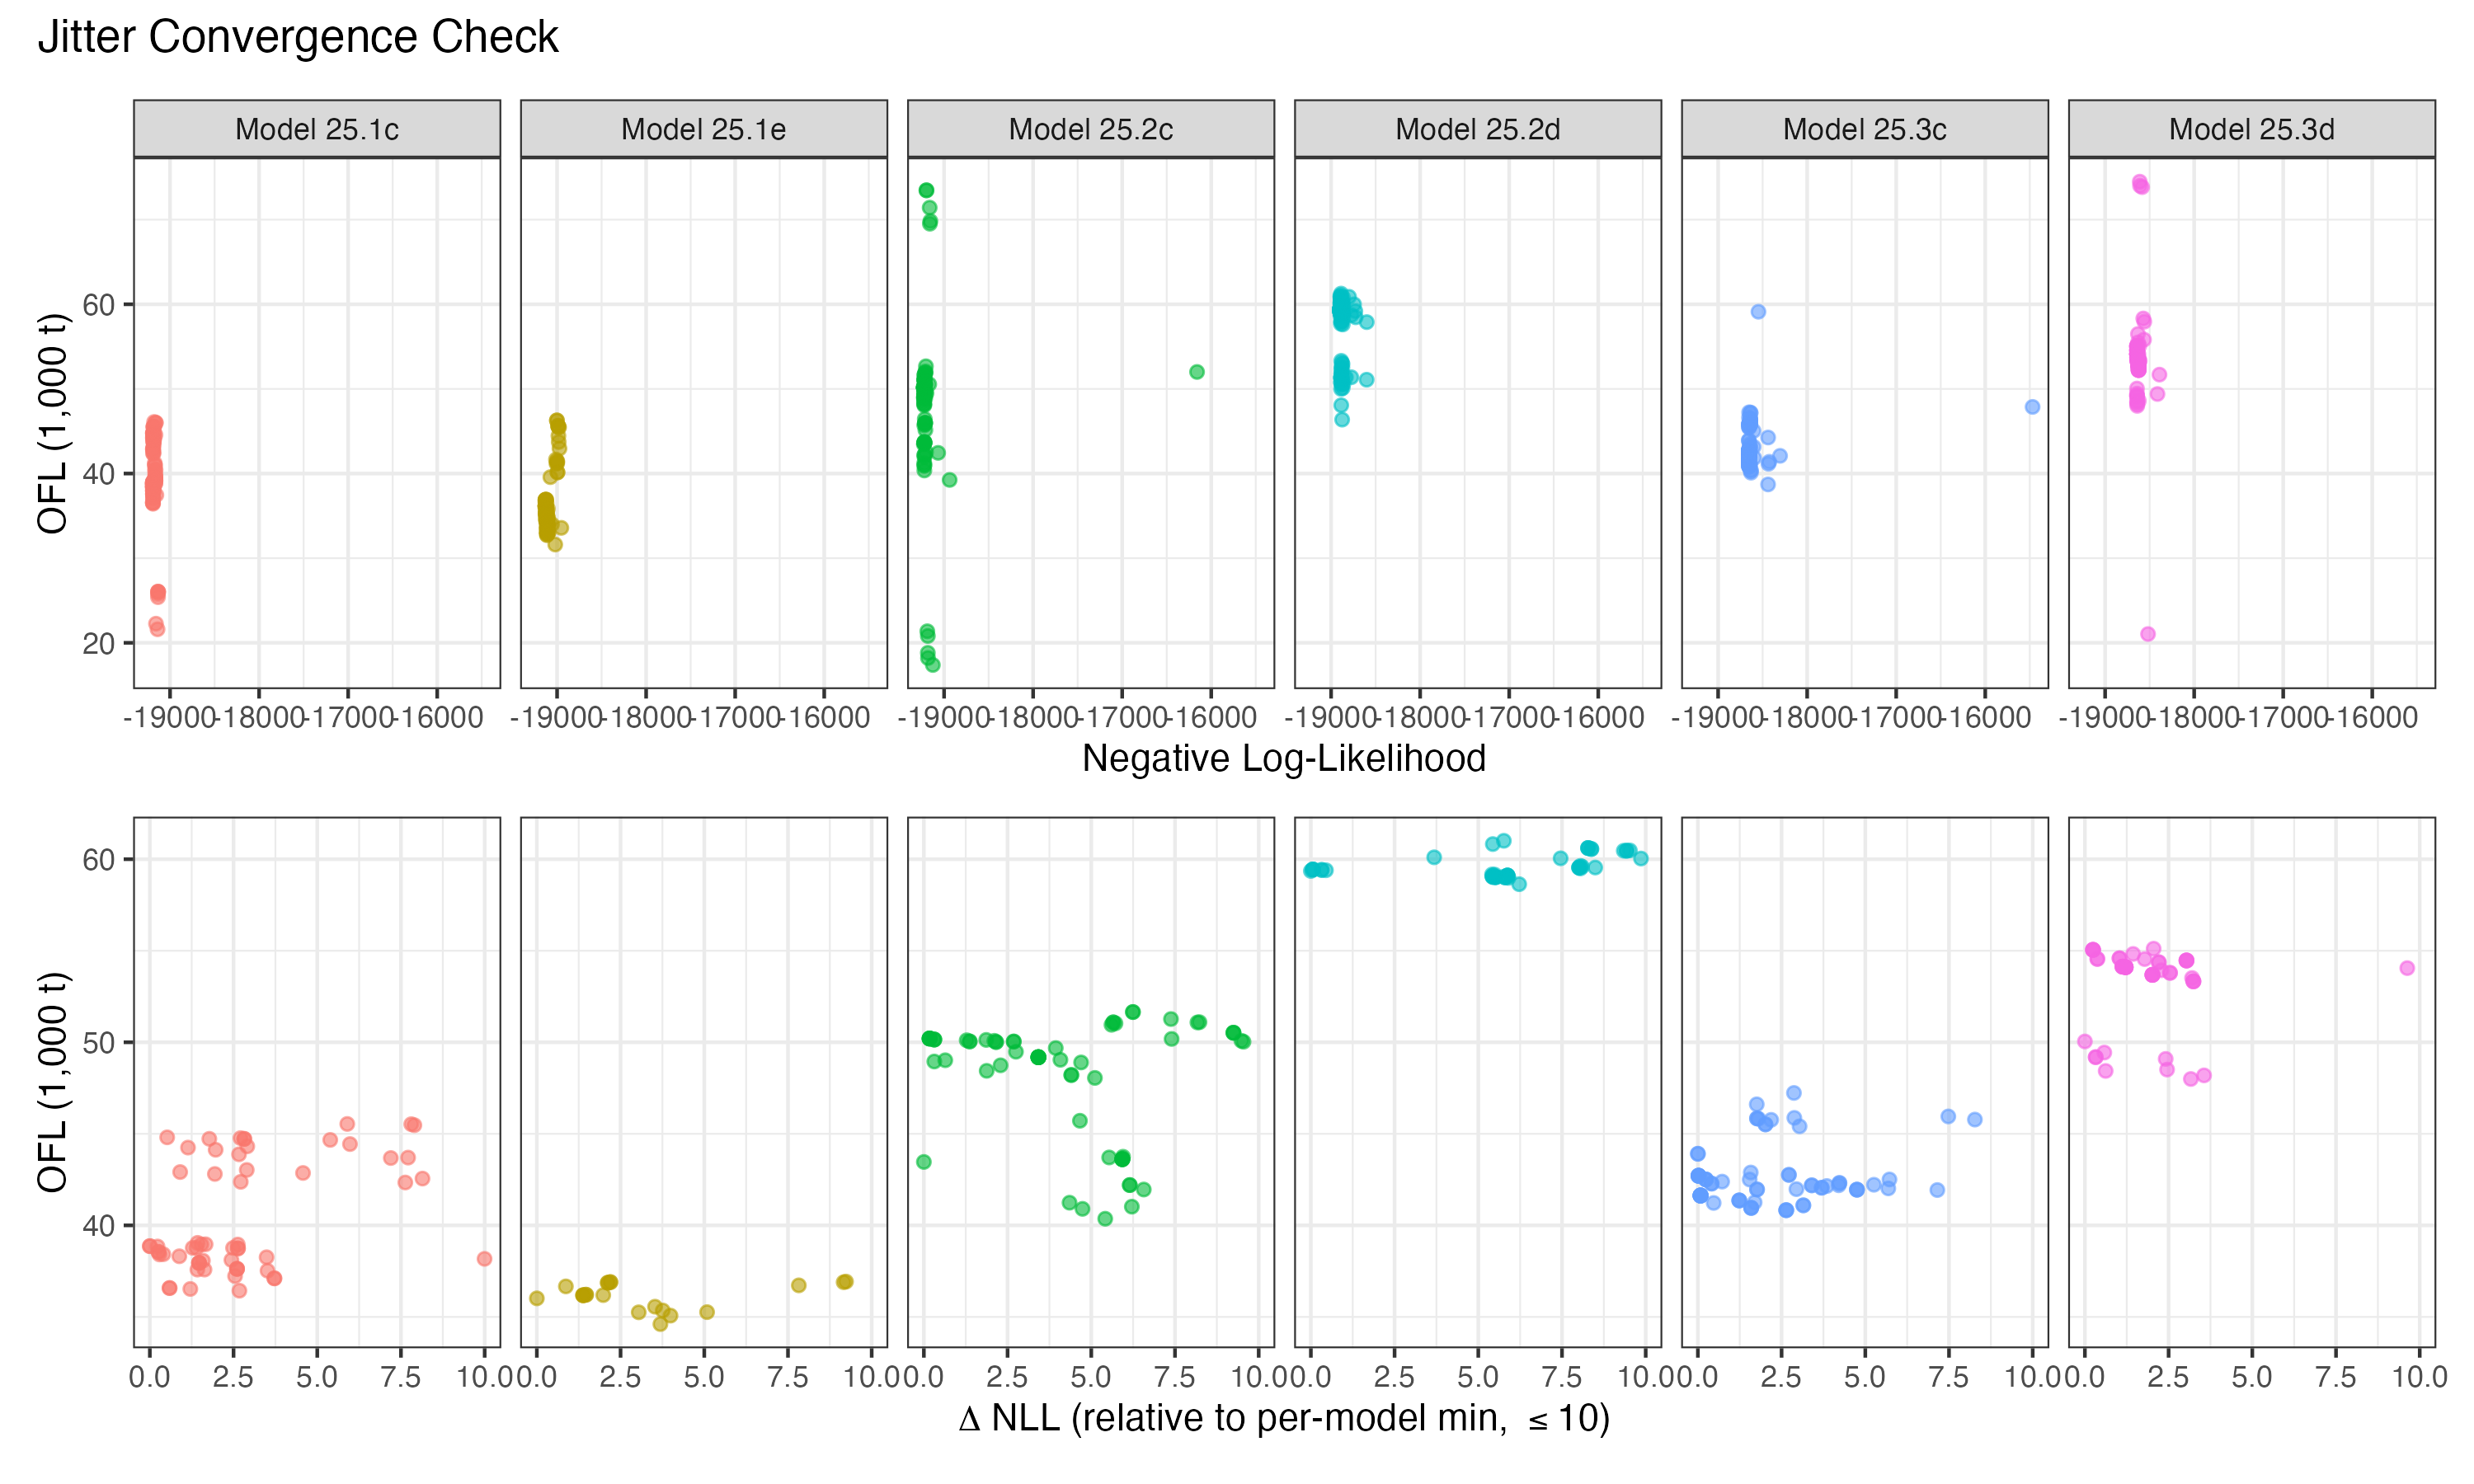
\includegraphics[height=0.55\textheight]{plots/jittered_results_ofl.png}
\tiny Directed Tier 3 OFL across 100 jitters per model (each point = one
converged jitter run).
\end{frame}

\begin{frame}{Jitter analysis -- 2024 male recruitment}
\phantomsection\label{jitter-analysis-2024-male-recruitment}
\centering

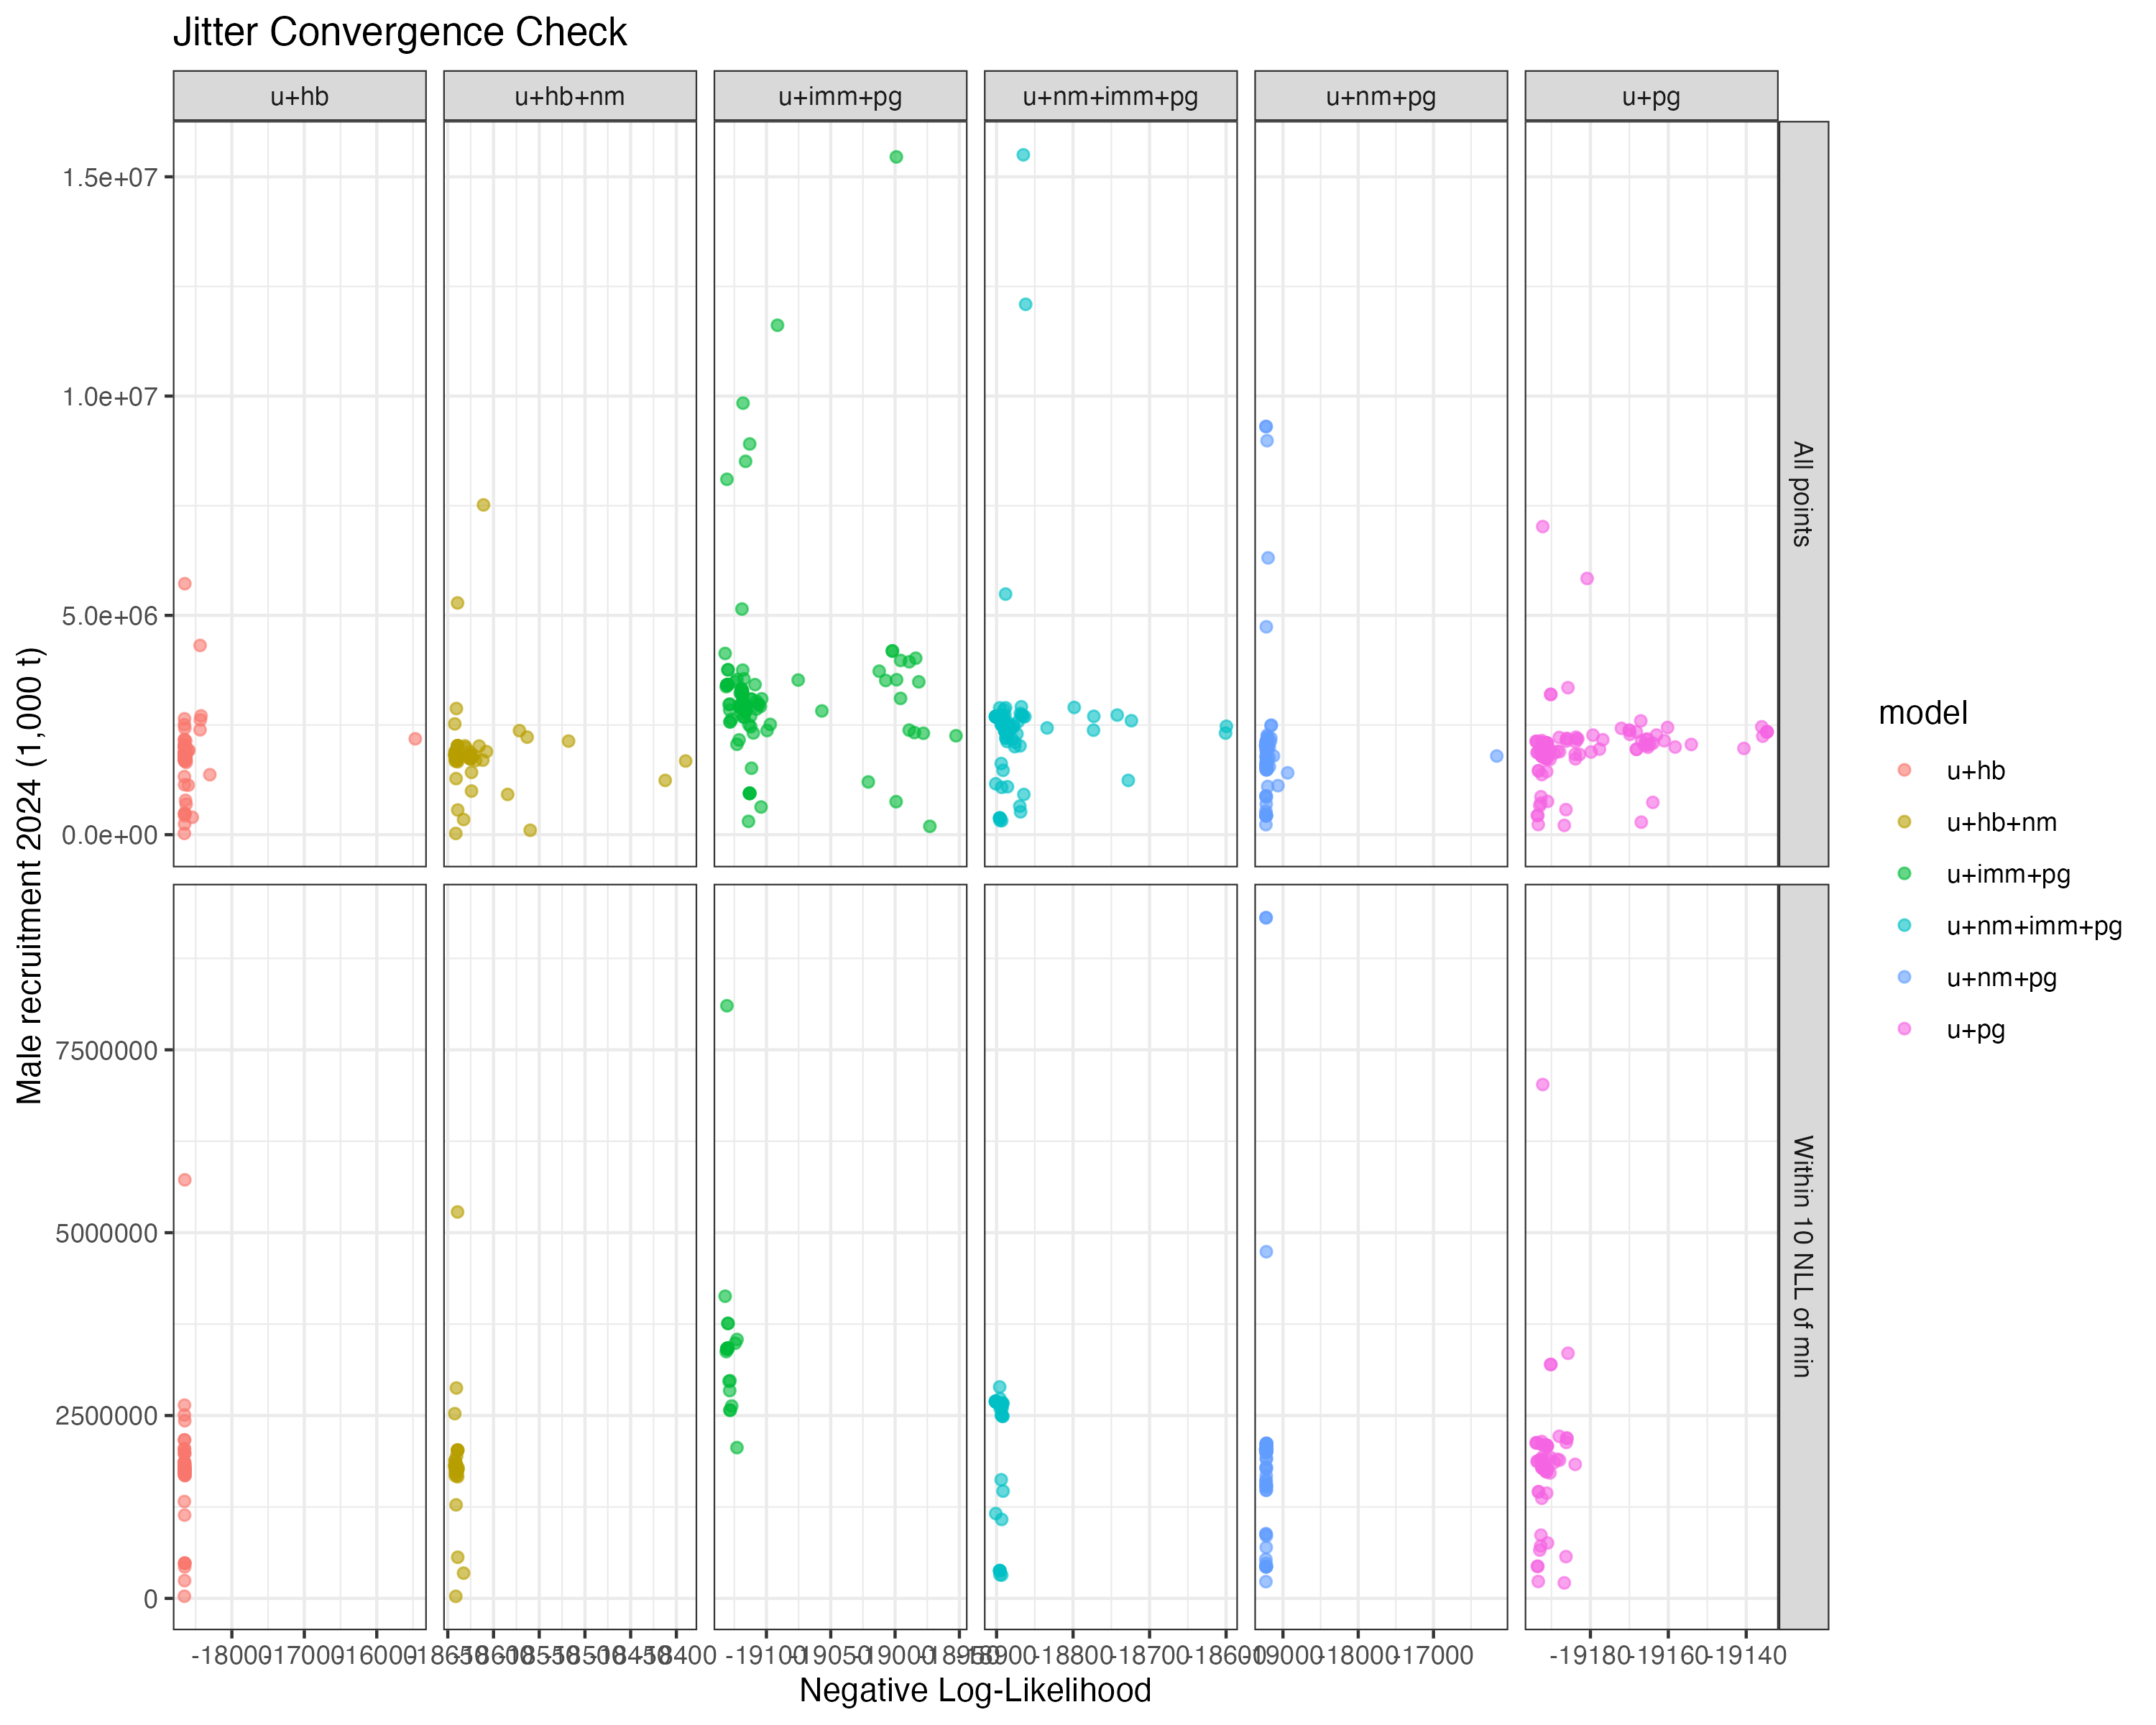
\includegraphics[height=0.7\textheight]{plots/jittered_results_rec.png}
\tiny Estimates of male recruitment in 2024 across 100 jitters;
vertically separated clouds indicate alternative local optima.
\end{frame}

\begin{frame}{Jitter analysis -- 2024 MMB}
\phantomsection\label{jitter-analysis-2024-mmb}
\centering

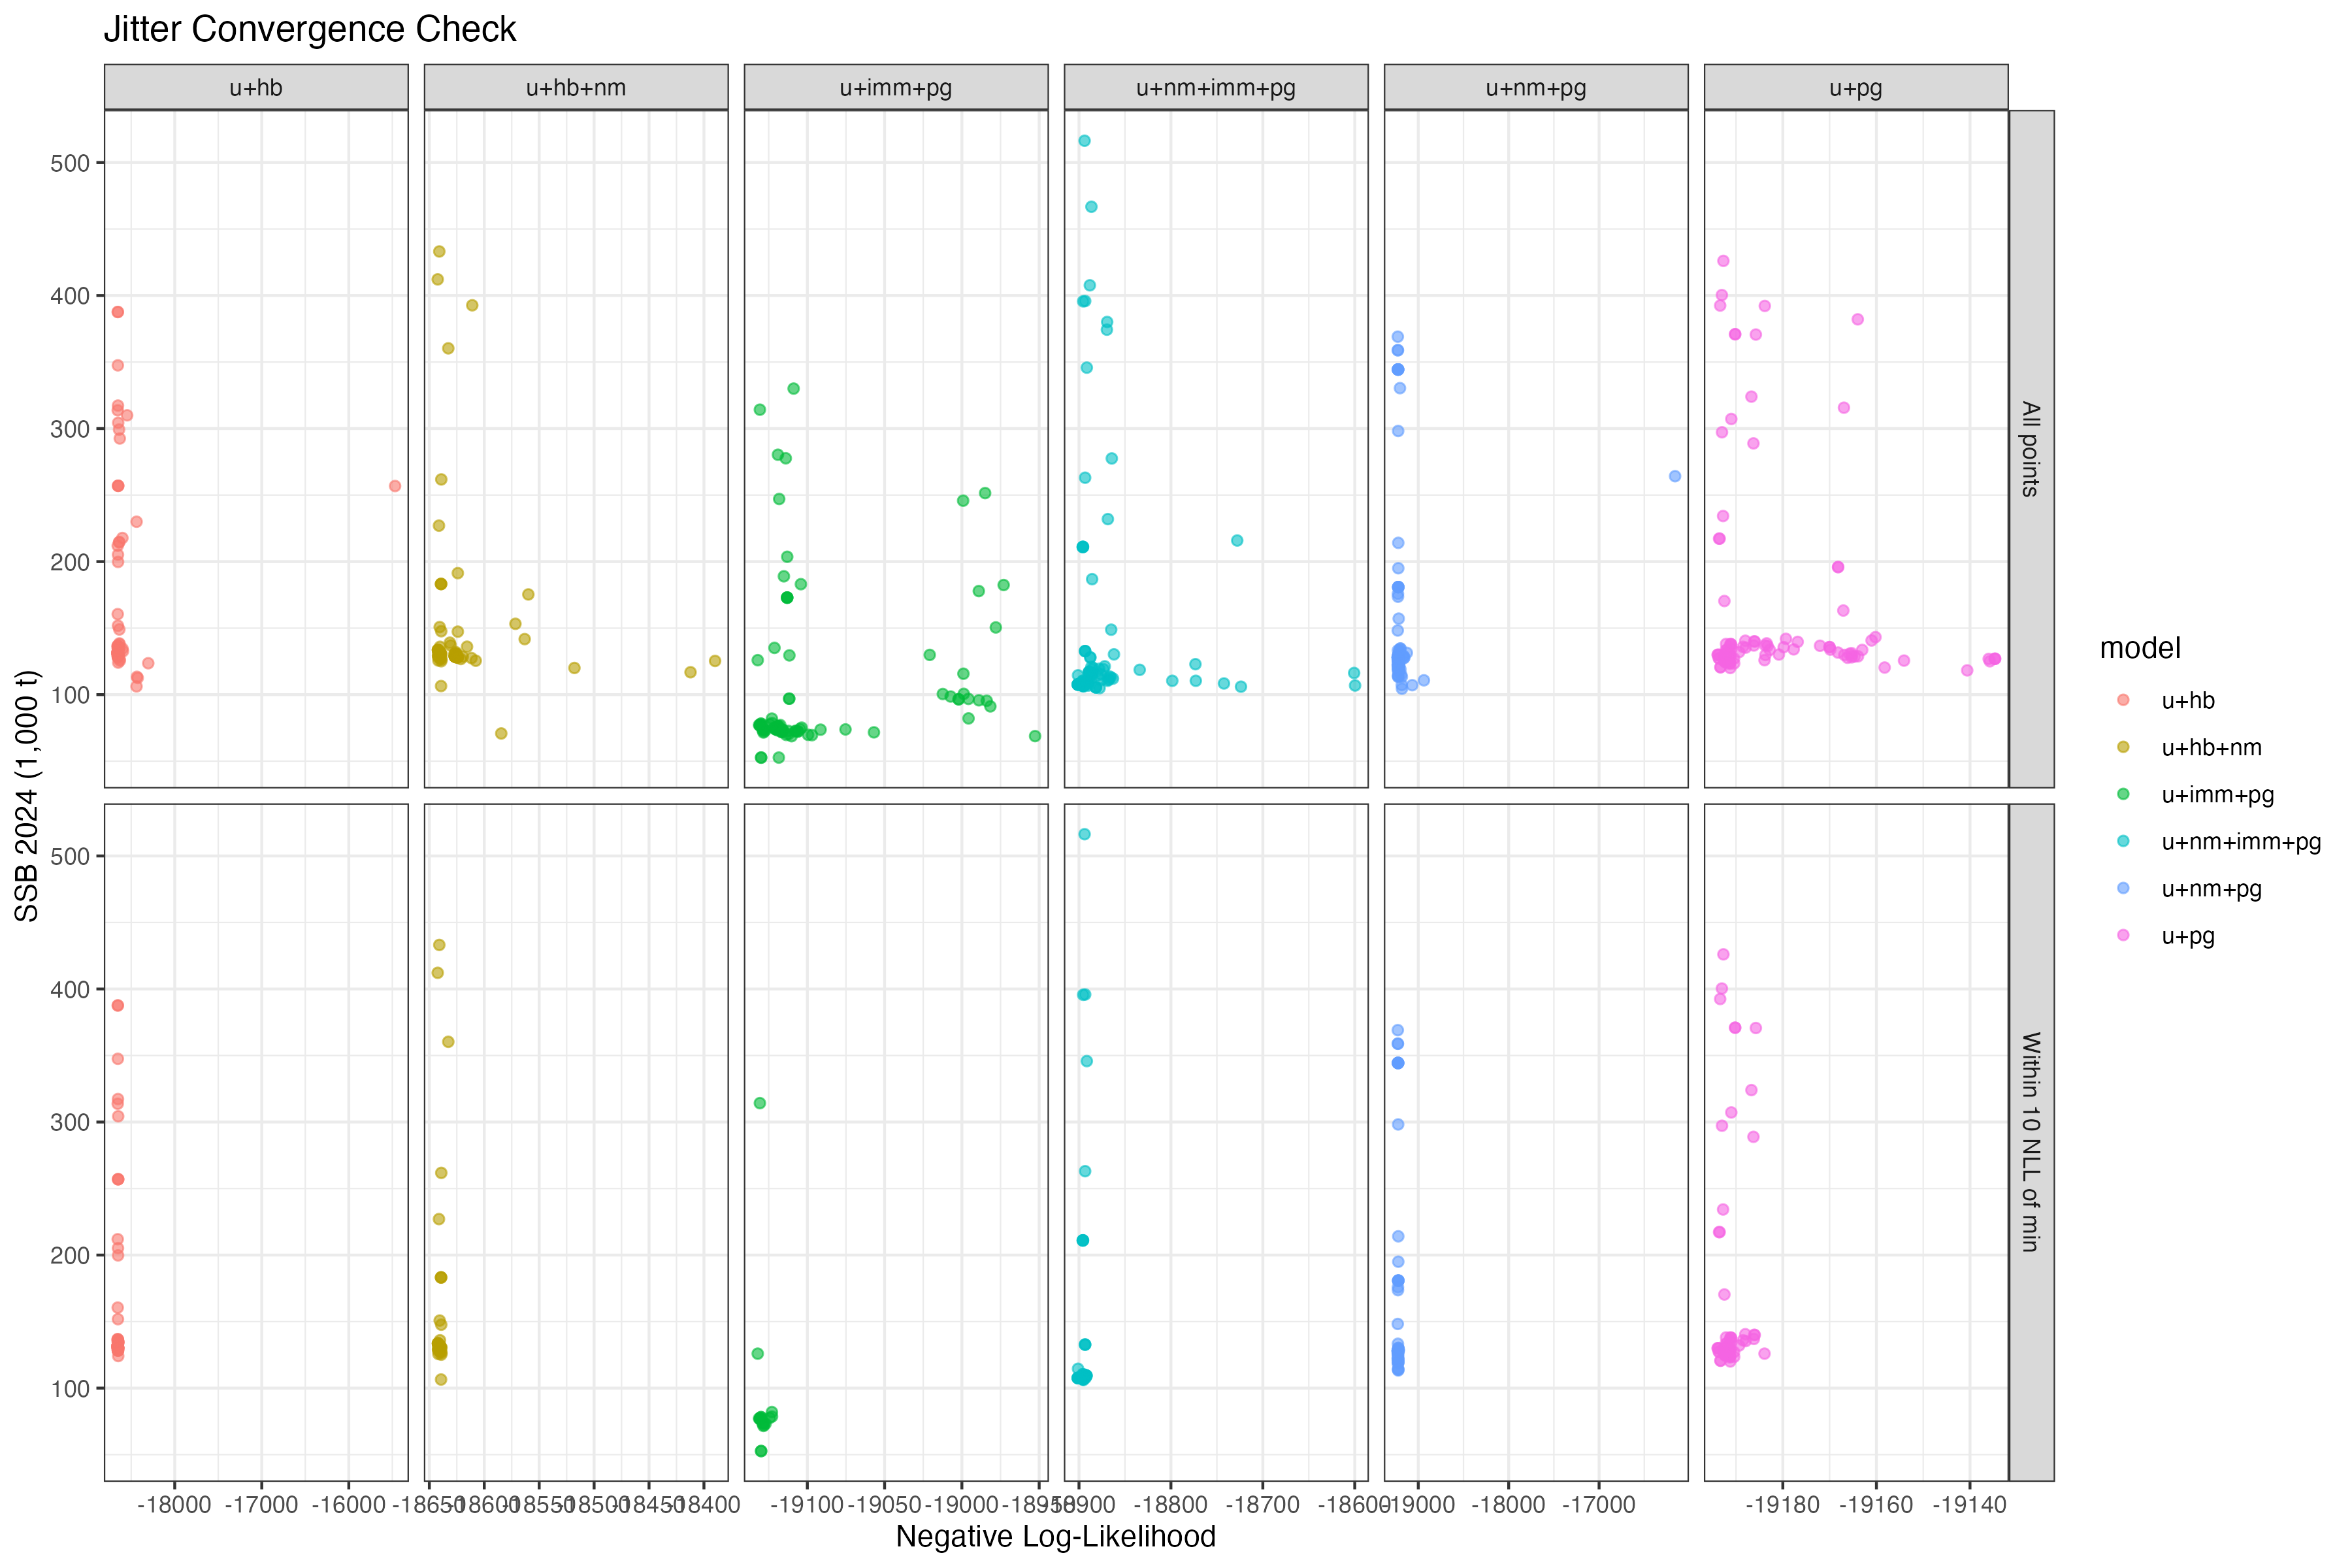
\includegraphics[height=0.7\textheight]{plots/jittered_results_ssb.png}
\tiny Estimates of MMB in 2024 across 100 jitters; bimodality dissolves
in models that include the immature survey index.
\end{frame}

\begin{frame}[fragile]{Interpreting the jitter results}
\phantomsection\label{interpreting-the-jitter-results}
\small

\begin{itemize}
\tightlist
\item
  \textbf{Adding the immature index alongside the updated plus group
  eliminates the bimodality} in OFL (\texttt{Model\ 25.1e},
  \texttt{Model\ 25.2d}).
\item
  A clear spread in derived quantities still exists within 10 NLL units,
  so \textbf{don't read this as an unqualified improvement}.
\item
  Bimodality has been a recurring issue in this assessment for several
  cycles.
\item
  Resolving the underlying source of multiple optima will require
  \textbf{further investigation} before September:

  \begin{itemize}
  \tightlist
  \item
    Which parameter combinations produce the two clouds?
  \item
    Recent recruitment? Mortality events? Selectivity?
  \item
    Does the immature index \emph{resolve} a real problem or \emph{mask}
    it?
  \end{itemize}
\end{itemize}
\end{frame}

\section{Model fits}\label{model-fits}

\begin{frame}{Fits to mature survey biomass}
\phantomsection\label{fits-to-mature-survey-biomass}
\small

\begin{itemize}
\tightlist
\item
  Fits to mature biomass survey indices broadly similar across models.
\item
  \textbf{All data-update candidates have difficulty fitting the
  terminal-year female biomass.} New maturity workflow shifts dynamics
  modestly but does not resolve this.
\item
  Hybrid-survey models have visibly higher predicted survey biomass in
  some years (additive hybrid biomass) but trends through time are
  unchanged.
\item
  Models with the immature survey index fit the new immature index well
  in recent years -- \emph{except} when paired with the new maturity
  ogive.
\end{itemize}
\end{frame}

\begin{frame}{Fits to size composition data -- key impressions}
\phantomsection\label{fits-to-size-composition-data-key-impressions}
\small

\begin{itemize}
\tightlist
\item
  \textbf{Retained males:} small differences across models. Plus-group
  change makes a small visual difference at the largest sizes.
\item
  \textbf{Total males:} noticeable differences between standard and
  hybrid-fishery models, particularly in the larger size bins where
  hybrids are most prevalent.
\item
  \textbf{Female discards (directed fishery):} no visually discernible
  differences across models.
\item
  \textbf{Non-directed fishery:} some of the largest misfits (single
  estimated selectivity, time-varying fishery behavior). Sample sizes
  assumed = 100 except 2021 and 2024 (=10).
\item
  \textbf{Survey size composition:} broadly similar fits across models.
  Persistent misfits for \textbf{immature females in 2009 and 2019} --
  could reflect unmodeled size-based mortality or time-varying
  probability of terminal molt.
\end{itemize}
\end{frame}

\begin{frame}{Example: total-male comp fits, hybrid vs.~non-hybrid}
\phantomsection\label{example-total-male-comp-fits-hybrid-vs.-non-hybrid}
\centering

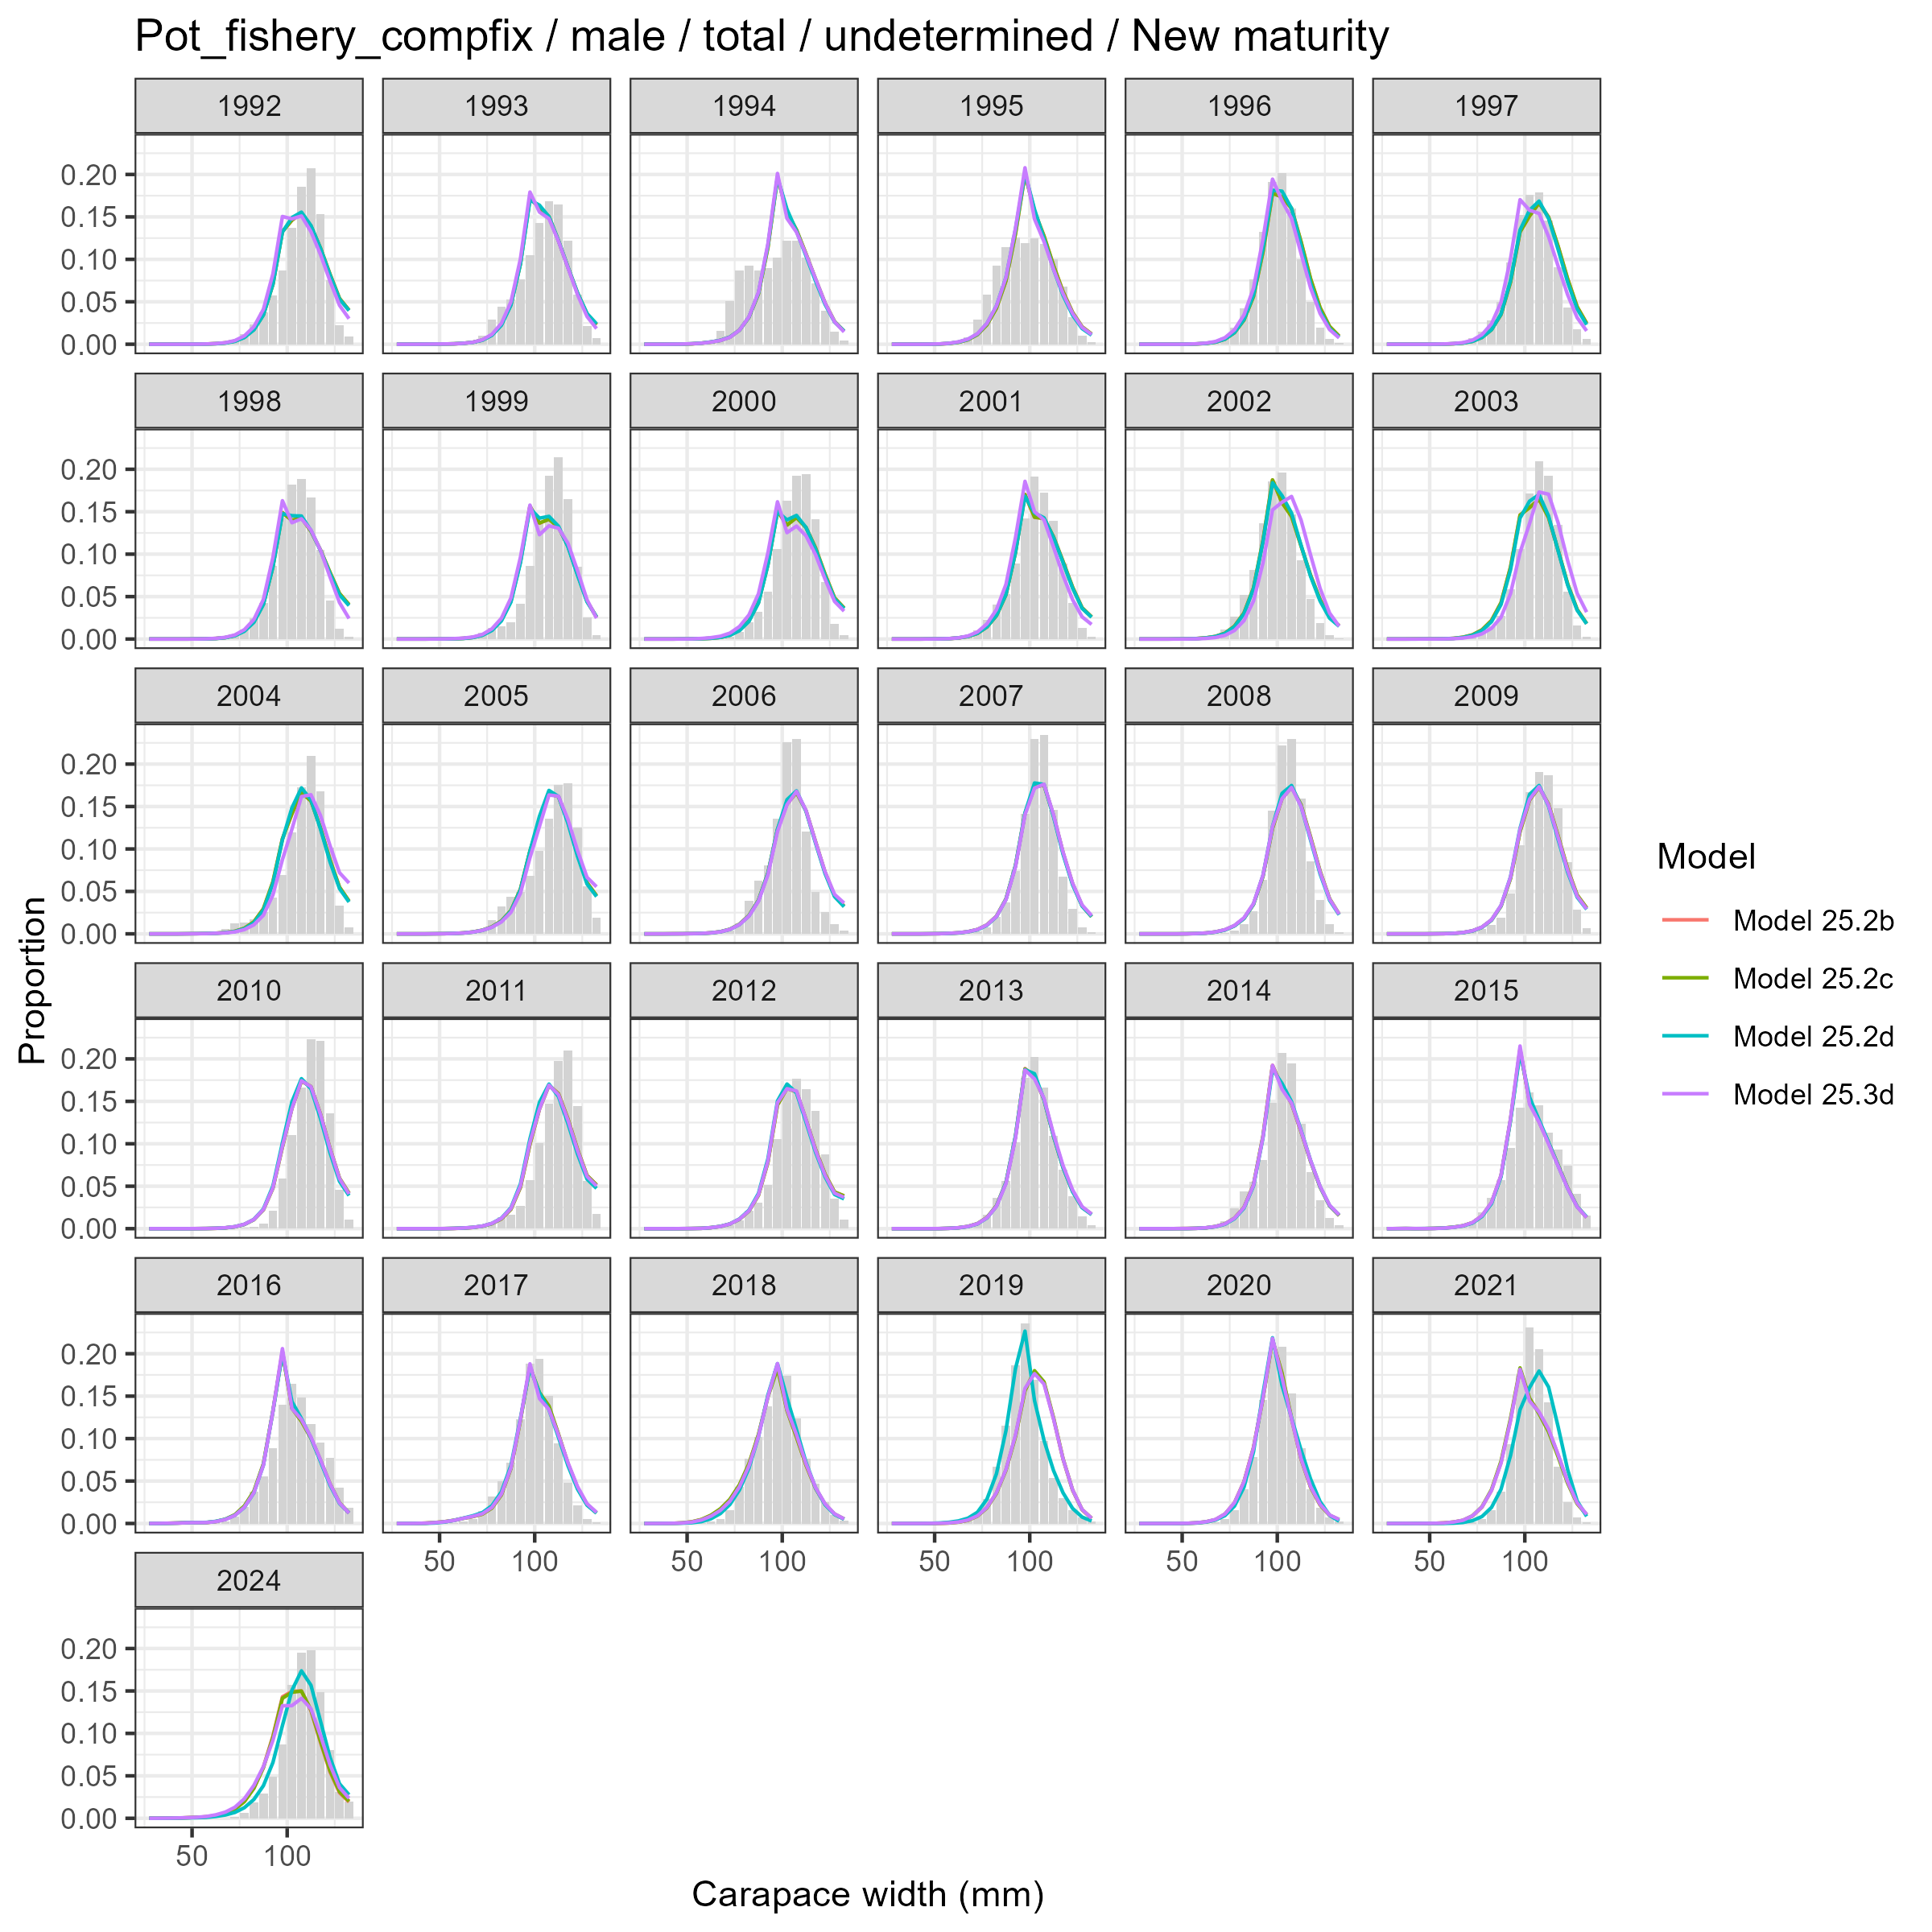
\includegraphics[height=0.78\textheight]{plots/size_comp_plot_41_Pot_fishery_compfix_male_total_undetermined_New_maturity.png}

\tiny Pot fishery total-male composition fits (compfix base, new
maturity); hybrid models fit the larger size bins more closely.
\end{frame}

\begin{frame}{Example: NMFS survey selectivity}
\phantomsection\label{example-nmfs-survey-selectivity}
\centering

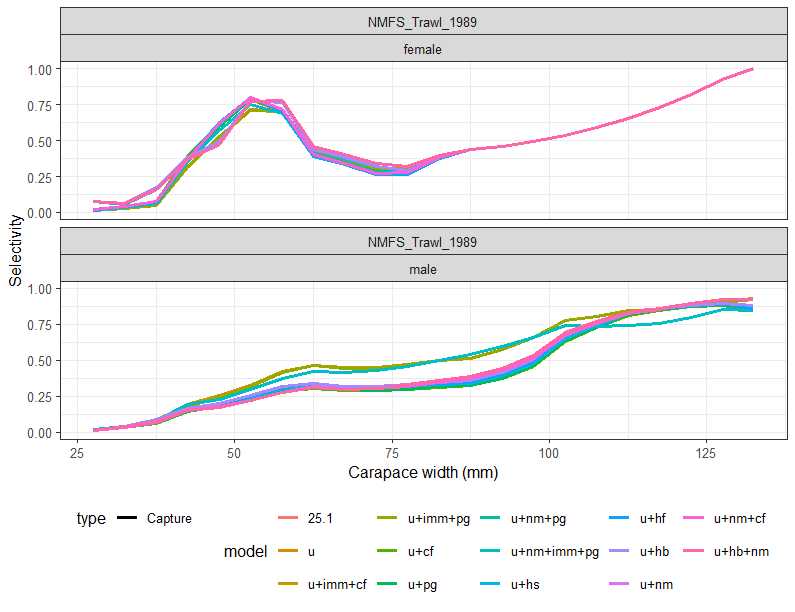
\includegraphics[height=0.7\textheight]{plots/survey_selex.png}
\tiny Estimated NMFS summer-trawl survey selectivity by era and sex with
BSFRF-derived priors. Recent-era estimates are similar across models.
\end{frame}

\section{Estimated population processes and
management}\label{estimated-population-processes-and-management}

\begin{frame}{Commercially preferred males (\textgreater=101 mm CW)}
\phantomsection\label{commercially-preferred-males-101-mm-cw}
\small

\begin{itemize}
\tightlist
\item
  Estimated abundance of commercially preferred male crab varies among
  models -- particularly in the early years where survey selectivity by
  era differs.
\item
  \textbf{All models agree}: abundance in recent years is at the
  \textbf{lowest in the time series}.
\item
  2025 survey biomass of preferred males = \textbf{23.28 kt}.
\item
  Most recent survey selectivity estimates are similar across models for
  both sexes.
\end{itemize}
\end{frame}

\begin{frame}[fragile]{Probability of terminal molt at size}
\phantomsection\label{probability-of-terminal-molt-at-size}
\small

\begin{itemize}
\tightlist
\item
  Probability of undergoing terminal molt is \textbf{input as data}.
\item
  \textbf{Legacy workflow:} strong increasing trend through time at
  intermediate sizes (at 77 mm: \textasciitilde0.2 in early 1990s
  \(\to\) \textasciitilde0.5 after 2010).
\item
  \textbf{New workflow (\texttt{sdmTMB}):} much weaker temporal trend
  (\textasciitilde0.35--0.45 throughout).
\item
  Difference in workflows propagates into the size composition data and
  the magnitude of recruitment to the fishery.
\end{itemize}

\medskip

\centering Implication: very different reference points and OFLs across
\texttt{Models\ 25.1*} vs.~\texttt{25.2*}.
\end{frame}

\begin{frame}{Recruitment}
\phantomsection\label{recruitment}
\small

\begin{itemize}
\tightlist
\item
  Recruitment trends very similar across models for the \textbf{early
  time series}, with some differences in scale and sex-specific timing.
\item
  Differences in \textbf{recent-year recruitment} are observed among
  models for males and contribute to differences in OFLs.
\item
  Sex-specific recruitment timing remains an open issue raised by the
  SSC -- see Author Responses.
\end{itemize}
\end{frame}

\begin{frame}[fragile]{Natural mortality}
\phantomsection\label{natural-mortality}
\small

\begin{itemize}
\tightlist
\item
  Base \(M\) for mature animals of both sexes is \textbf{broadly similar
  across models}, with one important exception:

  \begin{itemize}
  \tightlist
  \item
    \textbf{Models with the immature survey index produce substantially
    higher mature male \(M\)}, which propagates into smaller \(B_{MSY}\)
    and lower OFL.
  \end{itemize}
\item
  All models estimated additional mortality events removing \(\geq\)
  80\% of crab by sex/maturity (except mature females) at some point
  during the \textbf{2018--19 marine heatwave}.
\item
  \texttt{Model\ 25.3c} estimated immature female \(M\) above 100 in
  2019 (\textasciitilde600) -- much higher than other models. Suggests
  this configuration \textbf{should not be used to provide management
  advice}, or that females should be excluded from the management model.
\end{itemize}
\end{frame}

\begin{frame}[fragile]{MMB time series}
\phantomsection\label{mmb-time-series}
\small

\begin{itemize}
\tightlist
\item
  Trends in MMB are \textbf{similar across models}; \textbf{scales
  differ by up to \textasciitilde50\%} in some years.
\item
  Status (Bcurr/\(B_{MSY}\)) ranges 0.86--1.01 across the candidate set.
\item
  Hybrid-fishery and hybrid-both models produce slightly lower
  \(B_{MSY}\) proxies (\textasciitilde168--170 kt) than the
  corresponding non-hybrid, non-immature-index models
  (\textasciitilde172--181 kt) due to the additional fishing mortality.
\item
  New-maturity (no immature index) models cluster at
  \textasciitilde172--178 kt \(B_{MSY}\) but produce the \textbf{highest
  non-immature-index OFLs} (\textasciitilde50--52 kt) because the weaker
  time trend in \(\Pr\)(terminal molt) makes more crab available at
  fishery sizes.
\item
  Immature-index sensitivities (no new maturity) are outliers:
  \(B_{MSY}\) \textasciitilde94--96 kt, OFL \textasciitilde36 kt.
\item
  Combined immature-index + new-maturity (\texttt{Model\ 25.2d}):
  \textbf{highest OFL of the set (\textasciitilde60 kt)} at \(B_{MSY}\)
  = 163 kt; very large \(F_{MSY}\) and \(F_{OFL}\) (\textasciitilde71
  and \textasciitilde63).
\end{itemize}
\end{frame}

\begin{frame}[fragile]{Management quantities}
\phantomsection\label{management-quantities}
\centering
\tiny

\renewcommand{\arraystretch}{1.05}
\begin{tabular}{llrrrrr}
\toprule
\textbf{Model} & \textbf{Description} & \textbf{$B_{MSY}$} & \textbf{Bcurr/$B_{MSY}$} & \textbf{$F_{MSY}$} & \textbf{$F_{OFL}$} & \textbf{OFL} \\
 & & \textbf{(kt)} & & \textbf{(\%)} & \textbf{(\%)} & \textbf{(kt)} \\
\midrule
Model 25     & rolled fwd            & 180.1 & 0.88 & 39.5  & 34.4  & 44.3 \\

Model 25.1a  & update                & 184.8 & 0.86 & 35.9  & 30.5  & 44.0 \\
Model 25.1b  & compfix               & 177.5 & 0.90 & 41.7  & 37.2  & 45.9 \\

Model 25.1c  & + plus group          & 179.5 & 0.89 & 40.1  & 35.2  & 45.0 \\
Model 25.1d  & compfix + imm\_surv   & 94.3  & 0.95 & 157.5 & 149.3 & 36.4 \\

Model 25.1e  & plus + imm\_surv      & 96.0  & 0.98 & 152.3 & 148.7 & 34.8 \\
Model 25.2a  & new\_mat              & 171.9 & 0.97 & 38.2  & 36.8  & 51.4 \\

Model 25.2b  & compfix + new\_mat    & 173.5 & 0.96 & 39.5  & 37.9  & 51.5 \\
Model 25.2c  & plus + new\_mat       & 177.6 & 0.94 & 38.4  & 35.9  & 50.3 \\

Model 25.2d  & plus + new\_mat + imm & 163.4 & 0.90 & 70.9  & 63.1  & 59.5 \\
Model 25.3a  & plus + hyb\_fishery   & 169.3 & 0.91 & 37.0  & 33.4  & 44.2 \\

Model 25.3b  & plus + hyb\_surv      & 176.3 & 0.93 & 34.5  & 31.6  & 47.8 \\
Model 25.3c  & plus + hyb\_both      & 168.2 & 0.95 & 35.3  & 33.5  & 42.2 \\

Model 25.3d  & hyb\_both + new\_mat  & 169.8 & 1.01 & 44.1  & 44.1  & 49.6 \\
\bottomrule
\end{tabular}

\medskip

\tiny Values extracted from \texttt{Gmacsall.out} of each candidate run
(May 2026 fits).\textbackslash{} \tiny For reference: 2025 survey
commercially-preferred male biomass = \textbf{23.28 kt}.
\end{frame}

\begin{frame}{OFL summary}
\phantomsection\label{ofl-summary}
\small

\begin{itemize}
\tightlist
\item
  Tier 3 OFLs across the 14 candidates: \textbf{\textasciitilde36 to
  \textasciitilde60 kt}.
\item
  For reference, \textbf{2025 survey commercially-preferred male biomass
  = 23.28 kt}.
\item
  Differences driven by:

  \begin{enumerate}
  \tightlist
  \item
    Estimated \(M\) on mature males (highest in immature-index models).
  \item
    Time trend of \(\Pr\)(terminal molt) (legacy vs.~new maturity).
  \item
    Additional discard \(F\) implied by hybrid catches (lowers
    \(B_{MSY}\) slightly).
  \end{enumerate}
\item
  The immature-index sensitivities and the new-maturity sensitivities
  \textbf{bracket the candidate set}.
\item
  \textbf{Tier 4 fallback} will be presented in September following the
  standardized REMA-smoothed mature-male approach (October 2024 SSC).
\end{itemize}
\end{frame}

\begin{frame}{ABC buffer considerations}
\phantomsection\label{abc-buffer-considerations}
\small

\begin{itemize}
\tightlist
\item
  ABC = OFL \(\times\) (1 -- buffer).
\item
  SSC buffers used in recent years: \textbf{25\% (2025), 65\% (2024),
  50\% (2023), 25\% (2021), 25\% (2020)}.
\item
  Because \textbf{retained catch contains hybrids that cannot currently
  be separated} from snow crab, the assessment recommends that
  \textbf{the buffer accommodate the unknown retained-hybrid component}.
\item
  No author-recommended buffer is proposed at this time; this will be
  revisited in September with a smaller candidate set.
\end{itemize}
\end{frame}

\section{Author requests and
recommendations}\label{author-requests-and-recommendations}

\begin{frame}{Areas where the author seeks CPT/SSC guidance}
\phantomsection\label{areas-where-the-author-seeks-cptssc-guidance}
\small

This is a preliminary document. \textbf{No author-preferred model is
recommended.} The author seeks guidance on:

\begin{enumerate}
\tightlist
\item
  \textbf{Plus-group structural change} (\textgreater135 mm CW): faster,
  more interpretable size comp at the largest sizes, minimal change in
  management quantities. \emph{Author suggests adopting as the new
  structural baseline for September.}
\item
  \textbf{Inclusion of an immature survey index:} resolves bimodality,
  but produces a much larger mature-male \(M\). \emph{Will investigate
  biological credibility before September.}
\item
  \textbf{New maturity workflow:} weaker temporal trend in
  \(\Pr\)(terminal molt) than the legacy workflow. \emph{No strong
  preference; seeking guidance.}
\item
  \textbf{Hybrid treatment:} modest effect on management quantities;
  data-quality concerns flagged by ADF\&G in 1997--98. \emph{Author
  recommends one snow-only and one snow+hybrid (survey + fishery)
  sensitivity moving forward.}
\item
  \textbf{Convergence improvements:} none of the 14 candidates is fully
  clean. \emph{Author seeks guidance on what aspects of the model could
  be simplified} (male-only, fix \(M\), simpler survey selectivity).
\end{enumerate}
\end{frame}

\begin{frame}{Plan for September 2026}
\phantomsection\label{plan-for-september-2026}
\small

\begin{enumerate}
[(a)]
\item
  \textbf{Finalize structural choices} (plus group, maturity workflow,
  immature survey inclusion).
\item
  Update the \textbf{Tier 4 fallback} following the October 2024 SSC
  standardization.
\item
  \textbf{Investigate the high mature-male \(M\)} associated with the
  immature index -- biologically credible or model misspecification?
\item
  Complete \textbf{retrospective patterns} and \textbf{likelihood
  profiles} for the recommended models.
\item
  Update \textbf{rebuilding} and provide updated rebuilding timeline
  diagnostics.
\end{enumerate}
\end{frame}

\section{Data gaps and research
priorities}\label{data-gaps-and-research-priorities}

\begin{frame}[fragile]{Data gaps and research priorities}
\phantomsection\label{data-gaps-and-research-priorities-1}
\small

\begin{itemize}
\tightlist
\item
  \textbf{Hybrid identification consistency between ADF\&G and NMFS.}
  Different criteria for the number of secondary characteristics
  required for a positive hybrid identification.
\item
  \textbf{Apportionment of retained catch between snow and hybrids.}
  Currently retained catch contains both, with no method to partition.
\item
  \textbf{Quality control on early hybrid catch estimates.} 1997--98
  catches flagged by ADF\&G.
\item
  \textbf{Maturity workflow comparison.} Side-by-side documentation,
  sample-size diagnostics, and uncertainty quantification for the legacy
  vs.~\texttt{sdmTMB} workflows.
\item
  \textbf{Source of bimodality} in the snow crab assessment. Focused
  investigation to identify which parameter combinations produce the two
  clouds.
\item
  \textbf{Reproductive biology of large male snow crab.} Whether small
  males can produce progeny that become large males remains the central
  scientific uncertainty for management.
\end{itemize}
\end{frame}

\section{Acknowledgments}\label{acknowledgments}

\begin{frame}{Thank you}
\phantomsection\label{thank-you}
\centering
\Large

Tyler Jackson and Ben Daly (ADF\&G) -- hybrid catch, composition, and
discard data products

\bigskip

Erin Ryznar and the Kodiak lab -- new maturity workflow

\bigskip

André Punt, Buck Stockhausen, Matthieu Veron -- GMACS development

\bigskip

CPT and SSC -- comments and guidance

\bigskip

\normalsize

\textit{Questions and discussion welcome.}
\end{frame}

\section{Appendix}\label{appendix}

\begin{frame}[fragile]{Appendix: model -- file mapping}
\phantomsection\label{appendix-model-file-mapping}
\tiny

\begin{longtable}[]{@{}ll@{}}
\toprule\noalign{}
Model & Folder \\
\midrule\noalign{}
\endhead
Model 25 & \texttt{25\_gmacs/} \\
Model 25.1a & \texttt{25\_gmacs\_update/} \\
Model 25.1b & \texttt{25\_gmacs\_update\_compfix/} \\
Model 25.1c & \texttt{25\_gmacs\_update\_plus\_group/} \\
Model 25.1d & \texttt{25\_gmacs\_update\_imm\_compfix/} \\
Model 25.1e & \texttt{25\_gmacs\_update\_imm\_plus\_group/} \\
Model 25.2a & \texttt{25\_gmacs\_update\_newmat/} \\
Model 25.2b & \texttt{25\_gmacs\_update\_newmat\_compfix/} \\
Model 25.2c & \texttt{25\_gmacs\_update\_newmat\_plus\_group/} \\
Model 25.2d & \texttt{25\_gmacs\_update\_newmat\_imm\_plus\_group/} \\
Model 25.3a & \texttt{25\_gmacs\_update\_hyb\_fishery/} \\
Model 25.3b & \texttt{25\_gmacs\_update\_hyb\_surv/} \\
Model 25.3c & \texttt{25\_gmacs\_update\_hyb\_surv\_and\_fsh/} \\
Model 25.3d &
\texttt{25\_gmacs\_update\_hyb\_surv\_and\_fsh\_newmat/} \\
\bottomrule\noalign{}
\end{longtable}

\medskip

\scriptsize Repository:
\url{https://github.com/szuwalski/snow_crab/tree/dev-Grant}

Maturity workflow:
\url{https://github.com/eryznar/Chionoecetes.maturity.workflow}

GMACS: \url{https://github.com/GMACS-project}
\end{frame}




\end{document}
